\documentclass[%
  aspectratio=169,
  9pt,
  USenglish,
  titlegraphic, % store custom image to .images/titlegraphic
  affiliationintitlepagehead,
  %progressbar,
  affiliation,
]{beamer}

\usetheme{TUM}

\usepackage{tikz}  
\usepackage{tikz-3dplot} 
\usepackage{graphicx}
\usepackage{media9}
\usetikzlibrary{positioning}

\usepackage{amsmath}
\usepackage{booktabs}

% change the camera position
\tdplotsetmaincoords{45}{135}



\usepackage{animate}

\usepackage{pgfmath}
\newcommand\randmin{}
\newcommand\randmax{}
\newcommand\randmultof{}
\newcommand\setrand[4]%
{\def\randmin{#1}%
	\def\randmax{#2}%
	\def\randmultof{#3}%
	\pgfmathsetseed{#4}%
}
\newcommand\nextrand
{\pgfmathparse{int(int((rnd*(\randmax-\randmin+1)+\randmin)/\randmultof)*\randmultof)}%
	\xdef\thisrand{\pgfmathresult}%
}

%\usepackage[backend=biber]{biblatex}
%\addbibresource{bib/references.bib}

\newcommand{\wave}{
	\begin{tikzpicture}[xscale=.05,yscale=.2]
	\draw[-,fill=white] plot[domain=0:10*pi,smooth] (\x,{sin(\x r)});
	\end{tikzpicture}
}


\newcommand{\domain}[4]{
	%% spatial,spectral,temporal
	\draw[fill=#4, opacity=.2] (#1,0,0) -- (0,#2,0) -- (0,0,#3) -- (#1,0,0);
}


\newcommand{\radarwave}{
	\begin{tikzpicture}[xscale=.1,yscale=.2]
	\draw[-,fill=white] plot[domain=0:5*pi,smooth] (\x,{sin(\x r)});
	\end{tikzpicture}
}


\newcommand{\earth}{
	\begin{tikzpicture}[baseline=-.25em, inner sep=0]
	\node{
\includegraphics[width=8mm]{images/icons/earth}};
	\end{tikzpicture}
}

\newcommand{\sat}{
	\begin{tikzpicture}[baseline=-.25em, inner sep=0]
	\node[rotate=270,anchor=center]{
\includegraphics[width=8mm]{images/icons/sat2}};
	\end{tikzpicture}
}


\usepackage[capitalize]{cleveref}
\usepackage[square,sort,comma,numbers]{natbib}

%% this hack seems to be nececessary due to incompatibilities of cvpr template and tikz... -> https://tex.stackexchange.com/questions/398223/tikz-gives-error-command-everyshipouthook-already-defined
%\makeatletter
%\@namedef{ver@everyshi.sty}{}
%\makeatother
%% hackend

\usepackage{tikz}
\usepackage{pgfplots}
\usetikzlibrary{positioning, calc,arrows,arrows.meta, fit}
%\usetikzlibrary{arrows.meta,calc,decorations.markings,math,arrows.meta}
\usepgfplotslibrary{groupplots}
\usepgfplotslibrary{fillbetween}
\usepgfplotslibrary{statistics} % provides boxplots
\usepackage{xfrac}

\newcommand{\tp}{tp}
\newcommand{\tn}{tn}
\newcommand{\fp}{fp}
\newcommand{\fn}{fn}


\usepackage{tumcolors}
\usepackage{tummath}
\newcommand{\yhat}{\hat{\V{y}}}
\newcommand{\ycorrect}{\hat{y}^+}
\newcommand{\thetadelta}{\V{\Theta}_\delta}
\newcommand{\biasdelta}{b_\delta}
\newcommand{\biasclass}{\V{b}_\text{c}}
\newcommand{\thetaclass}{\V{\Theta}_\text{c}}
\newcommand{\thetafeat}{\V{\Theta}_\text{feat}}
\newcommand{\fclass}{f_\text{c}}
\newcommand{\fdelta}{f_\delta}
\newcommand{\ffeat}{f_\text{feat}}
\newcommand{\f}{f}

\newcommand{\rvtime}{T_c} 
\newcommand{\xuptot}{\M{X}_{\rightarrow t}} 
\newcommand{\deltauptot}{\delta_{\rightarrow t}} 
\newcommand{\tstop}{\ensuremath{t_\text{stop}}}
\newcommand{\meantstop}{\ensuremath{\bar{t}_\text{stop}}}
\usepackage[super]{nth}
\usepackage{mathtools}

\definecolor{evalcolor}{HTML}{3F3F3F}
\definecolor{traincolor}{HTML}{B98951}
\definecolor{validcolor}{HTML}{3F4BBE}

\definecolor{fdlcolor}{HTML}{142737}


\colorlet{colortrain}{tumblue}
\colorlet{colorinfer}{tumblack}

\colorlet{earlinesscolor}{tumblue}
\colorlet{accuracycolor}{tumorange}

\colorlet{stdcolor}{tumbluelight}
\colorlet{mediancolor}{tumorange}
\colorlet{meancolor}{tumblue}

\colorlet{b1color}{tumdiagramaubergine}
\colorlet{b2color}{tumdiagramnavyblue}
\colorlet{b3color}{tumdiagramturquoise}
\colorlet{b4color}{tumdiagramgreen}
\colorlet{b5color}{tumdiagramlimegreen}
\colorlet{b6color}{tumdiagramyellow}
\colorlet{b7color}{tumdiagramsand}
\colorlet{b8color}{tumdiagramredorange}
\colorlet{b8Acolor}{tumdiagramred}
\colorlet{b9color}{tumblack}
\colorlet{b10color}{tumblue}
\colorlet{b11color}{tumdiagramdarkred}
\colorlet{b12color}{tumorange}

% atmospheric bands
\colorlet{b1color}{tumblack}%tumdiagramaubergine
\colorlet{b9color}{tumblack}%tumblack
\colorlet{b10color}{tumblack}%tumblue

%visisble bands
\colorlet{b2color}{tumblue}%tumdiagramnavyblue
\colorlet{b3color}{tumblue}%tumdiagramturquoise
\colorlet{b4color}{tumblue}%tumdiagramgreen

% near infrared bands
\colorlet{b5color}{tumdiagramred}%tumdiagramlimegreen
\colorlet{b6color}{tumdiagramred}%tumdiagramyellow
\colorlet{b7color}{tumdiagramred}%tumdiagramsand
\colorlet{b8color}{tumdiagramred}%tumdiagramredorange
\colorlet{b8Acolor}{tumdiagramred}%tumdiagramred

% SWIR bands
\colorlet{b11color}{tumorange}%tumdiagramdarkred
\colorlet{b12color}{tumorange}%tumorange

\colorlet{epsilon0color}{tumorange}
\colorlet{epsilon1color}{tumblue}
\colorlet{epsilon10color}{tumblack}

\colorlet{gridcolor}{tumblue}
\colorlet{activationcolor}{tumorange}

\colorlet{meadowcolor}{tumbluemedium}
\colorlet{wbarleycolor}{tumbluedark}
\colorlet{corncolor}{tumorange}
\colorlet{wheatcolor}{tumgreen}
\colorlet{sbarleycolor}{tumdiagramred}
\colorlet{clovercolor}{tumdiagramturquoise}
\colorlet{triticalecolor}{tumdiagramsand}

\tikzstyle{rnn}=[draw,circle, inner sep=.1em]
\tikzstyle{norm}=[rounded corners,draw]
\tikzstyle{annot}=[rounded corners, fill=tumblue!20]
\tikzstyle{infer}=[-stealth, shorten >=.0em, shorten <=.0em, colorinfer]
\tikzstyle{loss}=[fill=tumblue!10, rounded corners, font=\small]
\tikzstyle{grad}=[colortrain]

\newcommand{\ptoffset}{\varepsilon}

\tikzstyle{test} = [thick]
\tikzstyle{train} = [thin, dotted]

\usepackage[inline]{enumitem}
\setenumerate{label=(\roman*),itemsep=3pt,topsep=3pt}

\setlength{\belowcaptionskip}{-10pt}


\colorlet{traincolor}{tumbluelight}
\colorlet{validcolor}{tumbluedark}
\colorlet{evalcolor}{tumorange}

\colorlet{forwardcolor}{tumblue}
\colorlet{backwardcolor}{tumorange}

% defaultvalue -> might be replaced later
\colorlet{tensorcolor}{forwardcolor}

\colorlet{classcolor}{tumivory}
\colorlet{encodercolor}{tumblue}
\colorlet{encodercolor}{tumblue}
\colorlet{colorblue}{tumblue}
\colorlet{colororange}{tumorange}

\colorlet{colorclassone}{tumblue}
\colorlet{colorclasstwo}{tumblack}
\colorlet{colorclassthree}{tumorange}
\colorlet{colorclassfour}{tumgray}

\colorlet{frh01color}{tumgray}
\colorlet{frh02color}{tumorange}
\colorlet{frh03color}{tumblue}
\colorlet{frh04color}{tumblack}



%\usepackage{media9}

% notation
\newcommand{\MWeight}{\ensuremath{\M{W}}}
\newcommand{\VBias}{\ensuremath{\V{b}}}
\newcommand{\VInput}{\DataVec}
\newcommand{\VHidden}{\ensuremath{\V{h}}}
\newcommand{\FActivation}{\ensuremath{\sigma}}
\newcommand{\VCellState}{\ensuremath{\V{c}}}
\newcommand{\VForgetGate}{\ensuremath{\V{f}}}
\newcommand{\VModulationGate}{\ensuremath{\V{j}}}
\newcommand{\VInputGate}{\ensuremath{\V{i}}}
\newcommand{\VOutputGate}{\ensuremath{\V{o}}}



\newcommand{\VResetGate}{\ensuremath{\V{r}}}
\newcommand{\VUpdateGate}{\ensuremath{\V{u}}}


%\usepackage{titlesec}
%\titlespacing{\section}{0pt}{10pt}{3pt}


\usetikzlibrary{3d}
\tikzstyle{perspective3d}=[
x={(0.5cm,0.5cm)}, y={(1cm,0cm)}, z={(0cm,1cm)}]


\usetikzlibrary{spy}

\usetikzlibrary{external,pgfplots.dateplot}

\usepackage[eulergreek]{sansmath}
\pgfplotsset{
	y tick label style={/pgf/number format/.cd,%
		scaled y ticks = false,
		set thousands separator={},
		fixed},
	x tick label style={/pgf/number format/.cd,%
		scaled x ticks = false,
		set decimal separator={,},
		fixed},
	tick label style = {font=\scriptsize\sansmath\sffamily},
	every axis label = {
		font=\scriptsize\sansmath\sffamily},
	every axis/.append style={
		axis lines=left, 
		enlargelimits, 
		thick},
	legend style = {font=\scriptsize\sansmath\sffamily, draw=none, rounded corners=0, fill opacity=.5, text opacity=1},
	label style = {font=\scriptsize\sansmath\sffamily},
	grid style={line width=.1pt, draw=gray!10},
	major grid style={line width=.2pt,draw=tumgraylight},
}

%\let\tempone\itemize
%\let\temptwo\enditemize
%\renewenvironment{itemize}{\tempone\addtolength{\itemsep}{-.5\baselineskip}}{\temptwo}

\tikzstyle{circ} = [circle, draw=white, fill=tumblue, inner sep=1pt]
\newcommand{\fcn}{
	\begin{tikzpicture}[scale=0.2, rotate=0, baseline=-.25em, inner sep=1pt]
	\node[circ](a0) at (0,-1){};
	\node[circ](a1) at (0,0){};
	\node[circ](a2) at (0,1){};
	
	\node[circ](b0) at (1,-0.5){};
	\node[circ](b1) at (1,0.5){};
	
	\draw[-] (a0) -- (b0);
	\draw[-] (a1) -- (b0);
	\draw[-] (a2) -- (b0);
	
	\draw[-] (a0) -- (b1);
	\draw[-] (a1) -- (b1);
	\draw[-] (a2) -- (b1);
	
	\end{tikzpicture}
}

\newcommand{\lfcn}[1]{
	\begin{tikzpicture}[scale=#1, rotate=0, baseline=-.25em, inner sep=1pt]
	\node[circle, draw=white, fill=tumblue, inner sep=3](a0) at (0,-1){};
	\node[circle, draw=white, fill=tumblue,  inner sep=3](a1) at (0,0){};
	\node[circle, draw=white, fill=tumblue,  inner sep=3](a2) at (0,1){};
	
	\node[circle, draw=white, fill=tumblue,  inner sep=3](b0) at (1,-0.5){};
	\node[circle, draw=white, fill=tumblue,  inner sep=3](b1) at (1,0.5){};
	
	\draw[-] (a0) -- (b0);
	\draw[-] (a1) -- (b0);
	\draw[-] (a2) -- (b0);
	
	\draw[-] (a0) -- (b1);
	\draw[-] (a1) -- (b1);
	\draw[-] (a2) -- (b1);
	
	\end{tikzpicture}
}

\newcommand{\hidden}[1]{
	\begin{tikzpicture}[scale=.1, baseline=-.25em]	
	%\draw[step=1.0,black,thin] (0,0) grid (#1,1);
	\foreach \i in {1,...,#1}{
		\node[circle, draw=white, fill=tumbluelight, inner sep=1pt] at (\i,0){};
	}
	\end{tikzpicture}
}

\newcommand{\drawvector}[1]{
	\begin{tikzpicture}[scale=.1, baseline=-.25em]	
	%\draw[step=1.0,black,thin] (0,0) grid (#1,1);
	\foreach \i in {1,...,#1}{
		\node[circ] at (\i,0){};
	}
	\end{tikzpicture}
}


\usetikzlibrary{external}
\tikzexternalize[prefix=tikz/]
\tikzexternalize
\tikzexternaldisable

\usepackage{tummath}

\setbeamertemplate{blocks}[rounded][shadow=false]
\usepackage{appendixnumberbeamer}

%	\end{itemize}
%	
%	Research Scope 
%	\begin{itemize}
%		\item Imbalance of Raster and Label Data
%		\item Analogies to NLP
%		\item Sequence modeling
%	\end{itemize}
%		
%	Research Projects
%	\begin{itemize}
%		\item Crop Classification with Multi-temporal Land Cover Classification
%		\item Early Classificaiton of Time Series
%	\end{itemize}
%		
%		
%\end{frame}


\title{BreizhCrops}
\subtitle{A Satellite Time Series Dataset for Crop Type Identification}
\author[M. Rußwurm, S. Lefèvre, M. Körner]{Marc Rußwurm,\footnotemark[1] Sébastien Lefèvre,\footnotemark[2] Marco Körner\footnotemark[1]}
\institute[TUM]{Technical Univ. of Munich, Remote Sensing Technology \footnotemark[1]  \\
IRISA-Obelix, University of South Brittany\footnotemark[2]}
\date{June 14th 2019, Time Series Workshop ICML 2019}

\begin{document}

\begin{frame}[t]
\titlepage
\end{frame}

{\setbeamercolor{background canvas}{bg=tumbluedark}
	\begin{frame}[plain]
	
	\vfill
	\Huge\color{white}
	\begin{center}
			We challenge the Time Series Community 
	\end{center}
	
	\vfill
\end{frame}
}

{\setbeamercolor{background canvas}{bg=white}
	\begin{frame}[plain]
	
	\vfill
	\Huge\color{tumbluedark}
	\begin{center}
		with a real-world time series dataset $\mathcal{D} = (\M{X},\V{y})^i$ \\
		\vspace{1em}
		\visible<2->{of satellite observations $\M{X} = (\V{x}_1^T,\V{x}_2^T,\dots,\V{x}_N^T)$} \\
		\vspace{1em}
		\visible<3->{vegetation classes $\V{y} = (y_\text{corn},y_\text{meadow},\dots)$}
		
	\end{center}
	
	\vfill
\end{frame}
}

{\setbeamercolor{background canvas}{bg=black}
	\begin{frame}[plain]
	
	\vfill
	\Huge\color{white}
	\begin{center}
		\begin{columns}
			\column{.5\textwidth}
			\vspace{7em}
			
			\hfill 
			Earth Observation
			\column{.5\textwidth}
			
			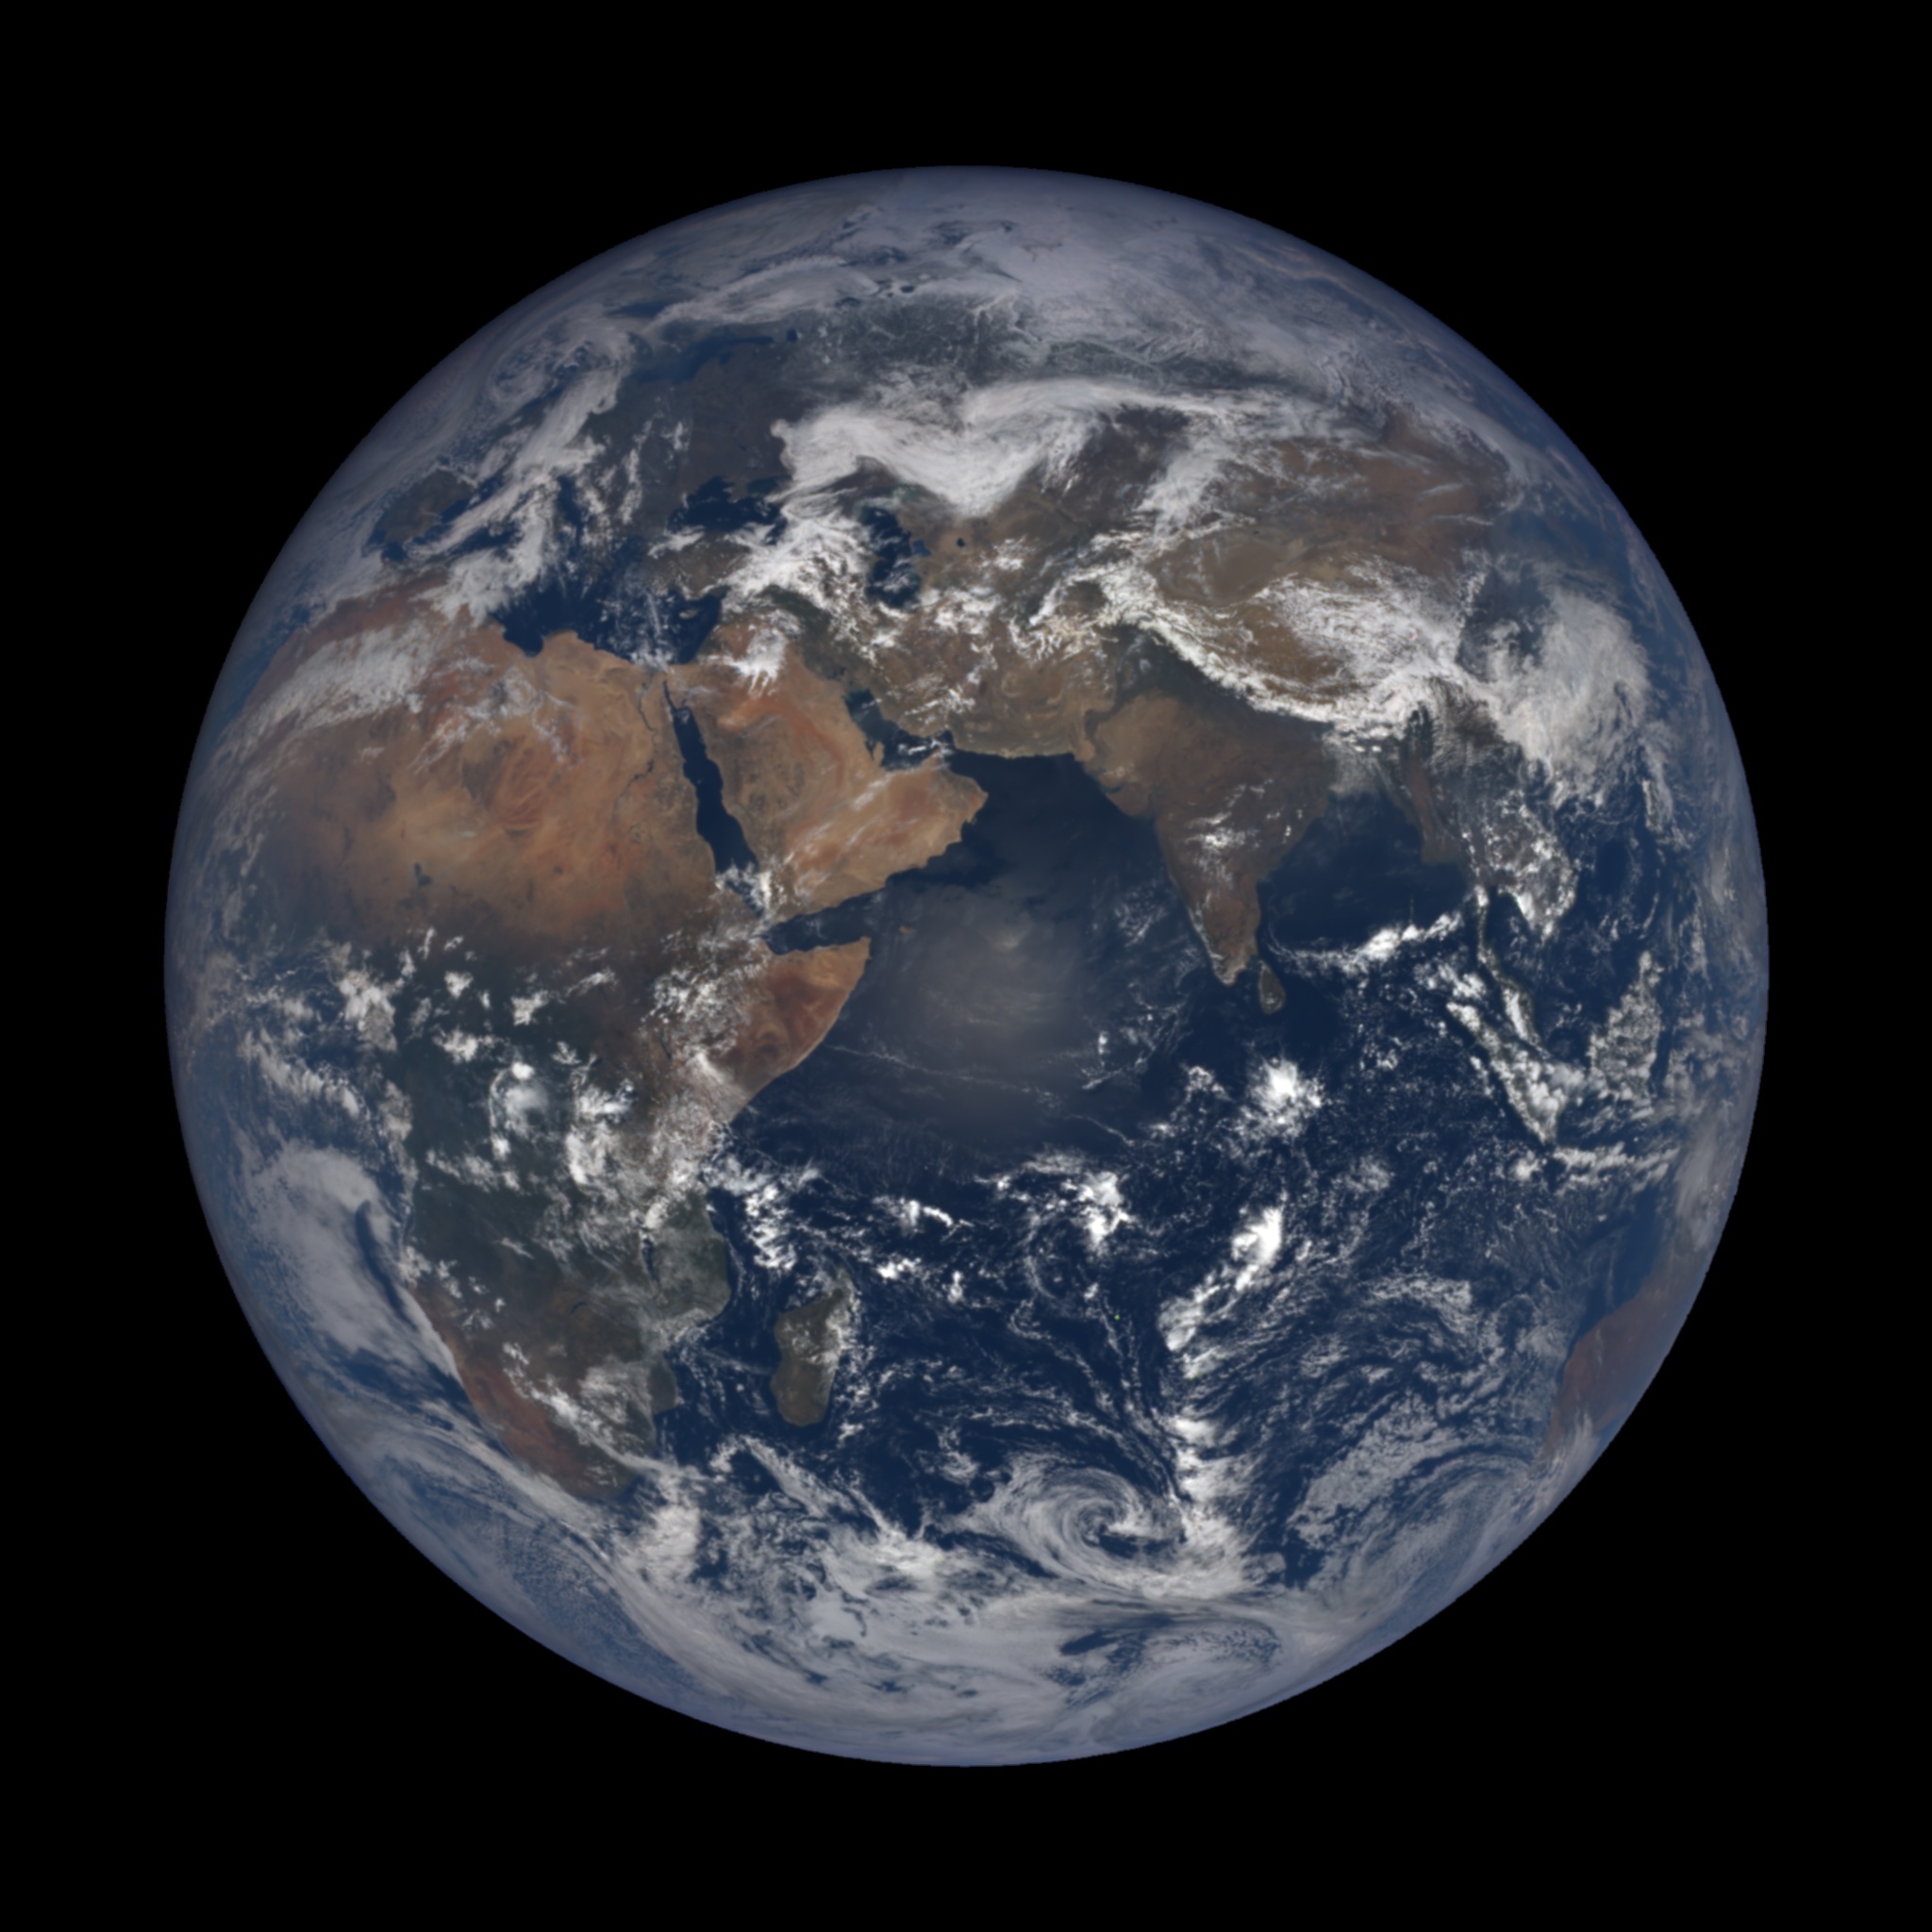
\includegraphics[width=5cm]{images/epic1}
			%\includegraphics[width=7cm]{images/fdl}
		\end{columns}
	\end{center}
	
	\vfill
\end{frame}
}

%
\begin{frame}
\frametitle{Optical Satellites}
\begin{columns}
	\column{.5\textwidth}
	
	
	\begin{itemize}[itemsep=.5em]
		\item<1-> Sensor measures \textbf{Digital Numbers} $\text{DN}(\lambda)$ for each wavelength $\lambda$. 
		\item<2-> \textbf{Digital Numbers} are normalized to \textbf{Radiance} 
		$L(\lambda), \left[\frac{W}{\text{sr}m^2}\right]$ by gain and offset calibration.
		\item<3-> Radiance is normalized to \textbf{top-of-atmosphere reflectance} $\rho(\lambda)$
%		\item<4-> \textbf{Bottom-of-atmosphere reflectances} are reconstructed using a functional model of the atmosphere.
	\end{itemize}
	
	%	Radiance $R_\lambda$ from measured Digital Numbers via calibrated gain $\alpha$ and offset $\beta$
	%	\begin{equation*}
	%		L_\lambda = \alpha \text{DN}_\lambda + \beta, \left[\frac{W}{\text{sr}m^1}\right]
	%	\end{equation*}
	%	
	%	top-of-atmosphere reflectance $\rho_\lambda$ as normalized Radiance $R_\lambda$ with solar 
	%	\begin{equation*}
	%	\rho_\lambda = \frac{L_\lambda}{\cos(\varphi_\text{sun})}
	%	\frac{
	%		\pi d^2
	%	}
	%	{
	%		E_\text{sun}(\lambda)
	%	}
	%	\end{equation*}
	%	
	%	\vspace{1em}
	%	
	%	\begin{itemize}
	%		\item measured radiance $L(\lambda)$
	%		\item solar irradiance $E_\text{sun}(\lambda)$
	%		\item solar zenith angle $\varphi_\text{sun}$
	%		\item squared Earth-Sun distance $d$ in AU
	%	\end{itemize}
	
	
	\column{.5\textwidth}
	
	
	\begin{tikzpicture}
	
	
	%	\draw [black,dotted, fill=tumbluelight,domain=110:70] plot ({13*cos(\x)}, {13*sin(\x)-12.8});
	\draw [fill=tumivory,domain=110:70] plot ({10*cos(\x)}, {10*sin(\x)-10});
	%	\draw [fill=tumbluelight,domain=110:70] plot ({12*cos(\x)}f, {12*sin(\x)-10});
	
	
	\node(sun) at (-2,2) {
\includegraphics[width=10mm]{images/icons/sun}};
	\node[rotate=130,anchor=center](sat) at (2,2) {
\includegraphics[width=10mm]{images/icons/sat2}};
	
	\node(px) at ({10*cos(90)}, {10*sin(90)-10.1}){
		\begin{tikzpicture}[xscale=.5,yscale=.25]
		\draw[fill=tumbluelight] (0,0) -- (1,0) -- (2,1) -- (1,1) -- (0,0);
		\end{tikzpicture}
		%
\includegraphics[width=5mm]{images/icons/house}
	};
	
	\draw[-stealth] (sun) -- node[midway,sloped]{\wave} (px);
	\draw[-stealth] (px) -- node[midway,sloped]{\wave} (sat);
	
	\visible<3->{\draw[-stealth] (sun) -- node[midway,sloped]{\wave} (sat);
		\draw[draw=tumgray] (px) -- node[at end,left]{$\varphi_\text{sun}$} ++(0,1.4); 
		\draw [draw=tumgray, domain=130:90] plot ({1*cos(\x)}, {1*sin(\x)});
	}
	
	\node[above=.5em of sun]{$E_\text{sun}(\lambda)$};
	\visible<1>{\node[above=4em of sat]{$DN(\lambda)$};}
	\visible<2>{\node[above=4em of sat]{$L(\lambda)$};}
	\visible<3>{\node[above=4em of sat]{$\rho_\text{toa}(\lambda)$};}
%	\visible<4>{\node[above=4em of sat]{$\rho_\text{boa}(\lambda)$};}
	
	%		\draw[red] (0,0) sin (1,2);
	
\end{tikzpicture}
\end{columns}
\end{frame}

\begin{frame}
	\frametitle{Acquired in regular time intervals}
	\framesubtitle{Sentinel 2 Satellite}
	
%	\includemovie[
%	poster,
%	text={\small(Loading Circle-m-increase3.mp4)}
%	]{6cm}{6cm}{images/s2orbits.mp4}
%	
%	\movie{loaded}{images/s2orbits.avi}
	
	\begin{columns}
		\column{.5\textwidth}
		
		\Large
		\begin{itemize}
			\item<1-> polar sun-synchronous orbit
			\item<2-> single orbit circa 100 minutes
			\item<3-> revisit same location after 5 days
			\item<4-> acquisition stripe of 290km width
			\item<5-> 13 spectral bands
			\item<6-> ground resolution 10-60m
			\item<7-> global coverage and free of charge
		\end{itemize}
		
		\column{.5\textwidth}
%		\only<1>{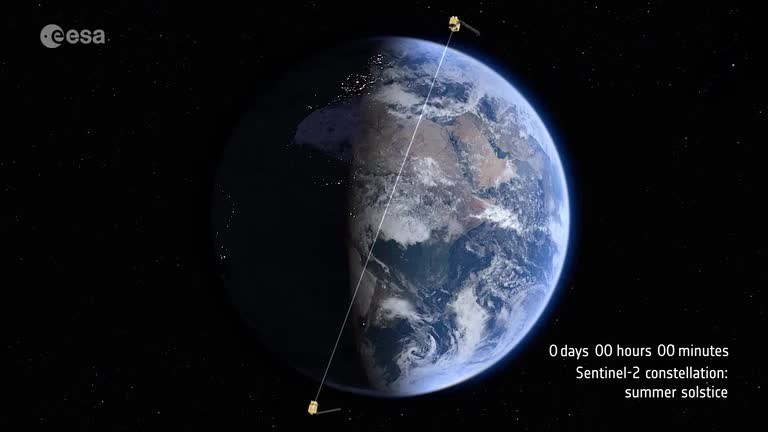
\includegraphics[width=\textwidth]{images/s2orbits/1}}
%		\only<2>{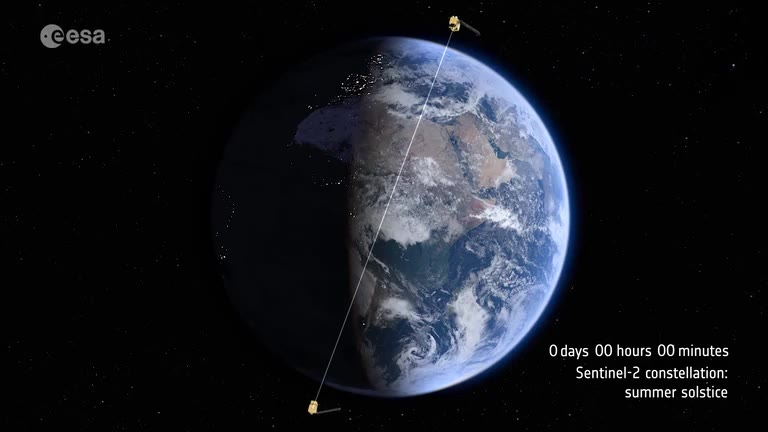
\includegraphics[width=\textwidth]{images/s2orbits/2}}
%		\only<3>{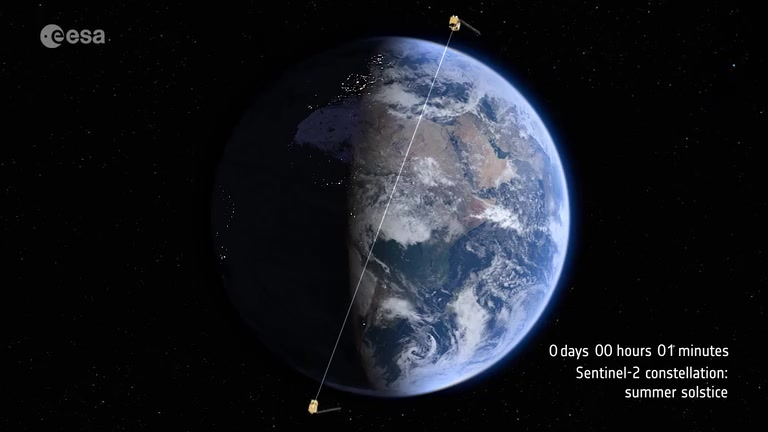
\includegraphics[width=\textwidth]{images/s2orbits/3}}
		\only<1>{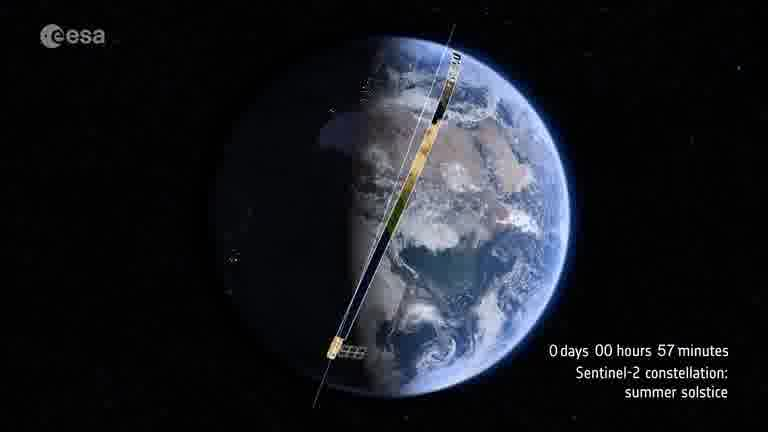
\includegraphics[width=\textwidth]{images/s2orbits/14}}
		\only<2>{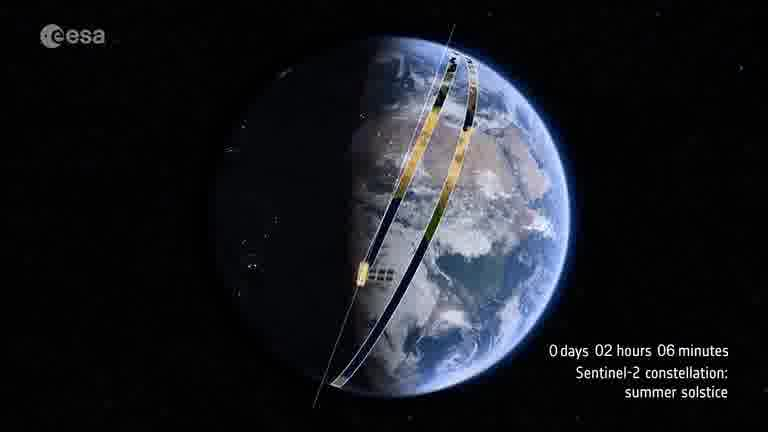
\includegraphics[width=\textwidth]{images/s2orbits/19}}
		\only<3>{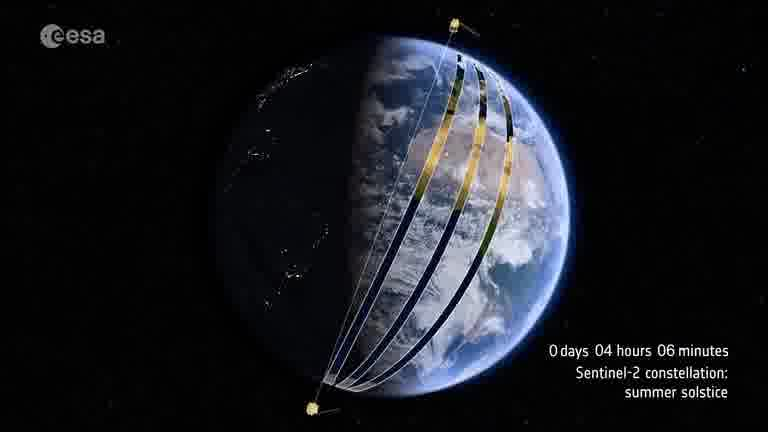
\includegraphics[width=\textwidth]{images/s2orbits/24}}
		\only<4>{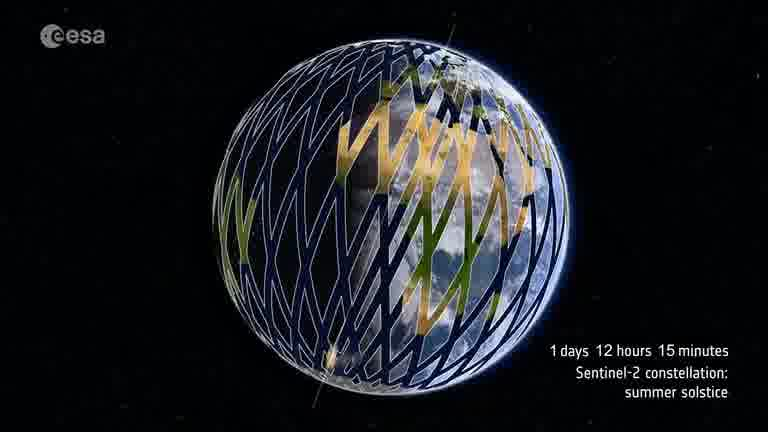
\includegraphics[width=\textwidth]{images/s2orbits/35}}
		\only<5>{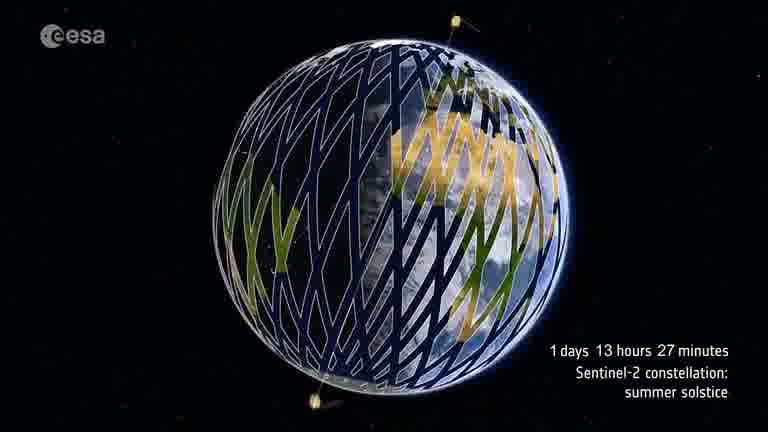
\includegraphics[width=\textwidth]{images/s2orbits/36}}
		\only<6>{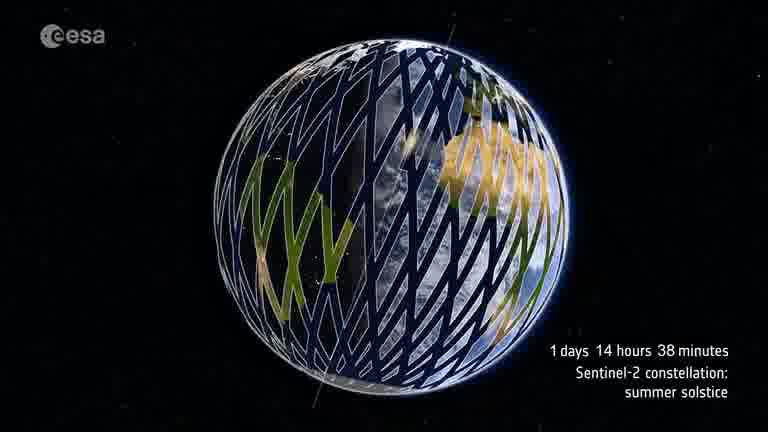
\includegraphics[width=\textwidth]{images/s2orbits/37}}
		\only<7>{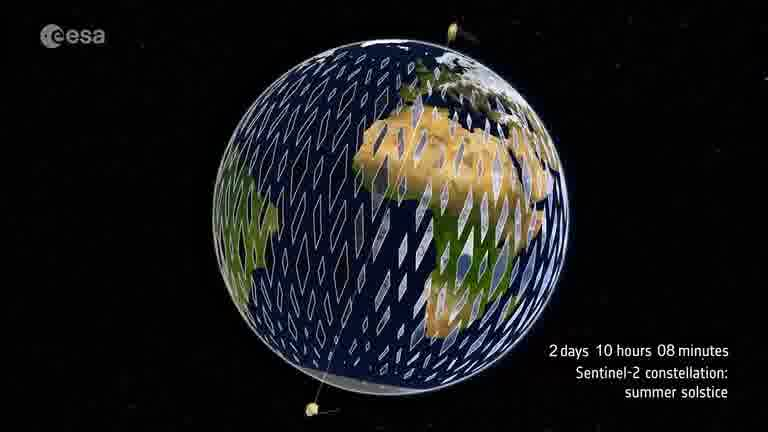
\includegraphics[width=\textwidth]{images/s2orbits/48}}
		\tiny\url{https://www.esa.int/spaceinvideos/Videos/2016/08/Sentinel-2_global_coverage}
	\end{columns}
	
\end{frame}
%
%
%{\setbeamercolor{background canvas}{bg=tumblack}
%	\begin{frame}[plain]
%	
%	\vfill
%	\Huge\color{white}
%	\begin{center}
%		\begin{columns}
%			\column{.5\textwidth}
%			\vspace{7em}
%			
%			\hfill 
%			Satellite Data Take-away
%			\column{.5\textwidth}
%			
%			
%			%%			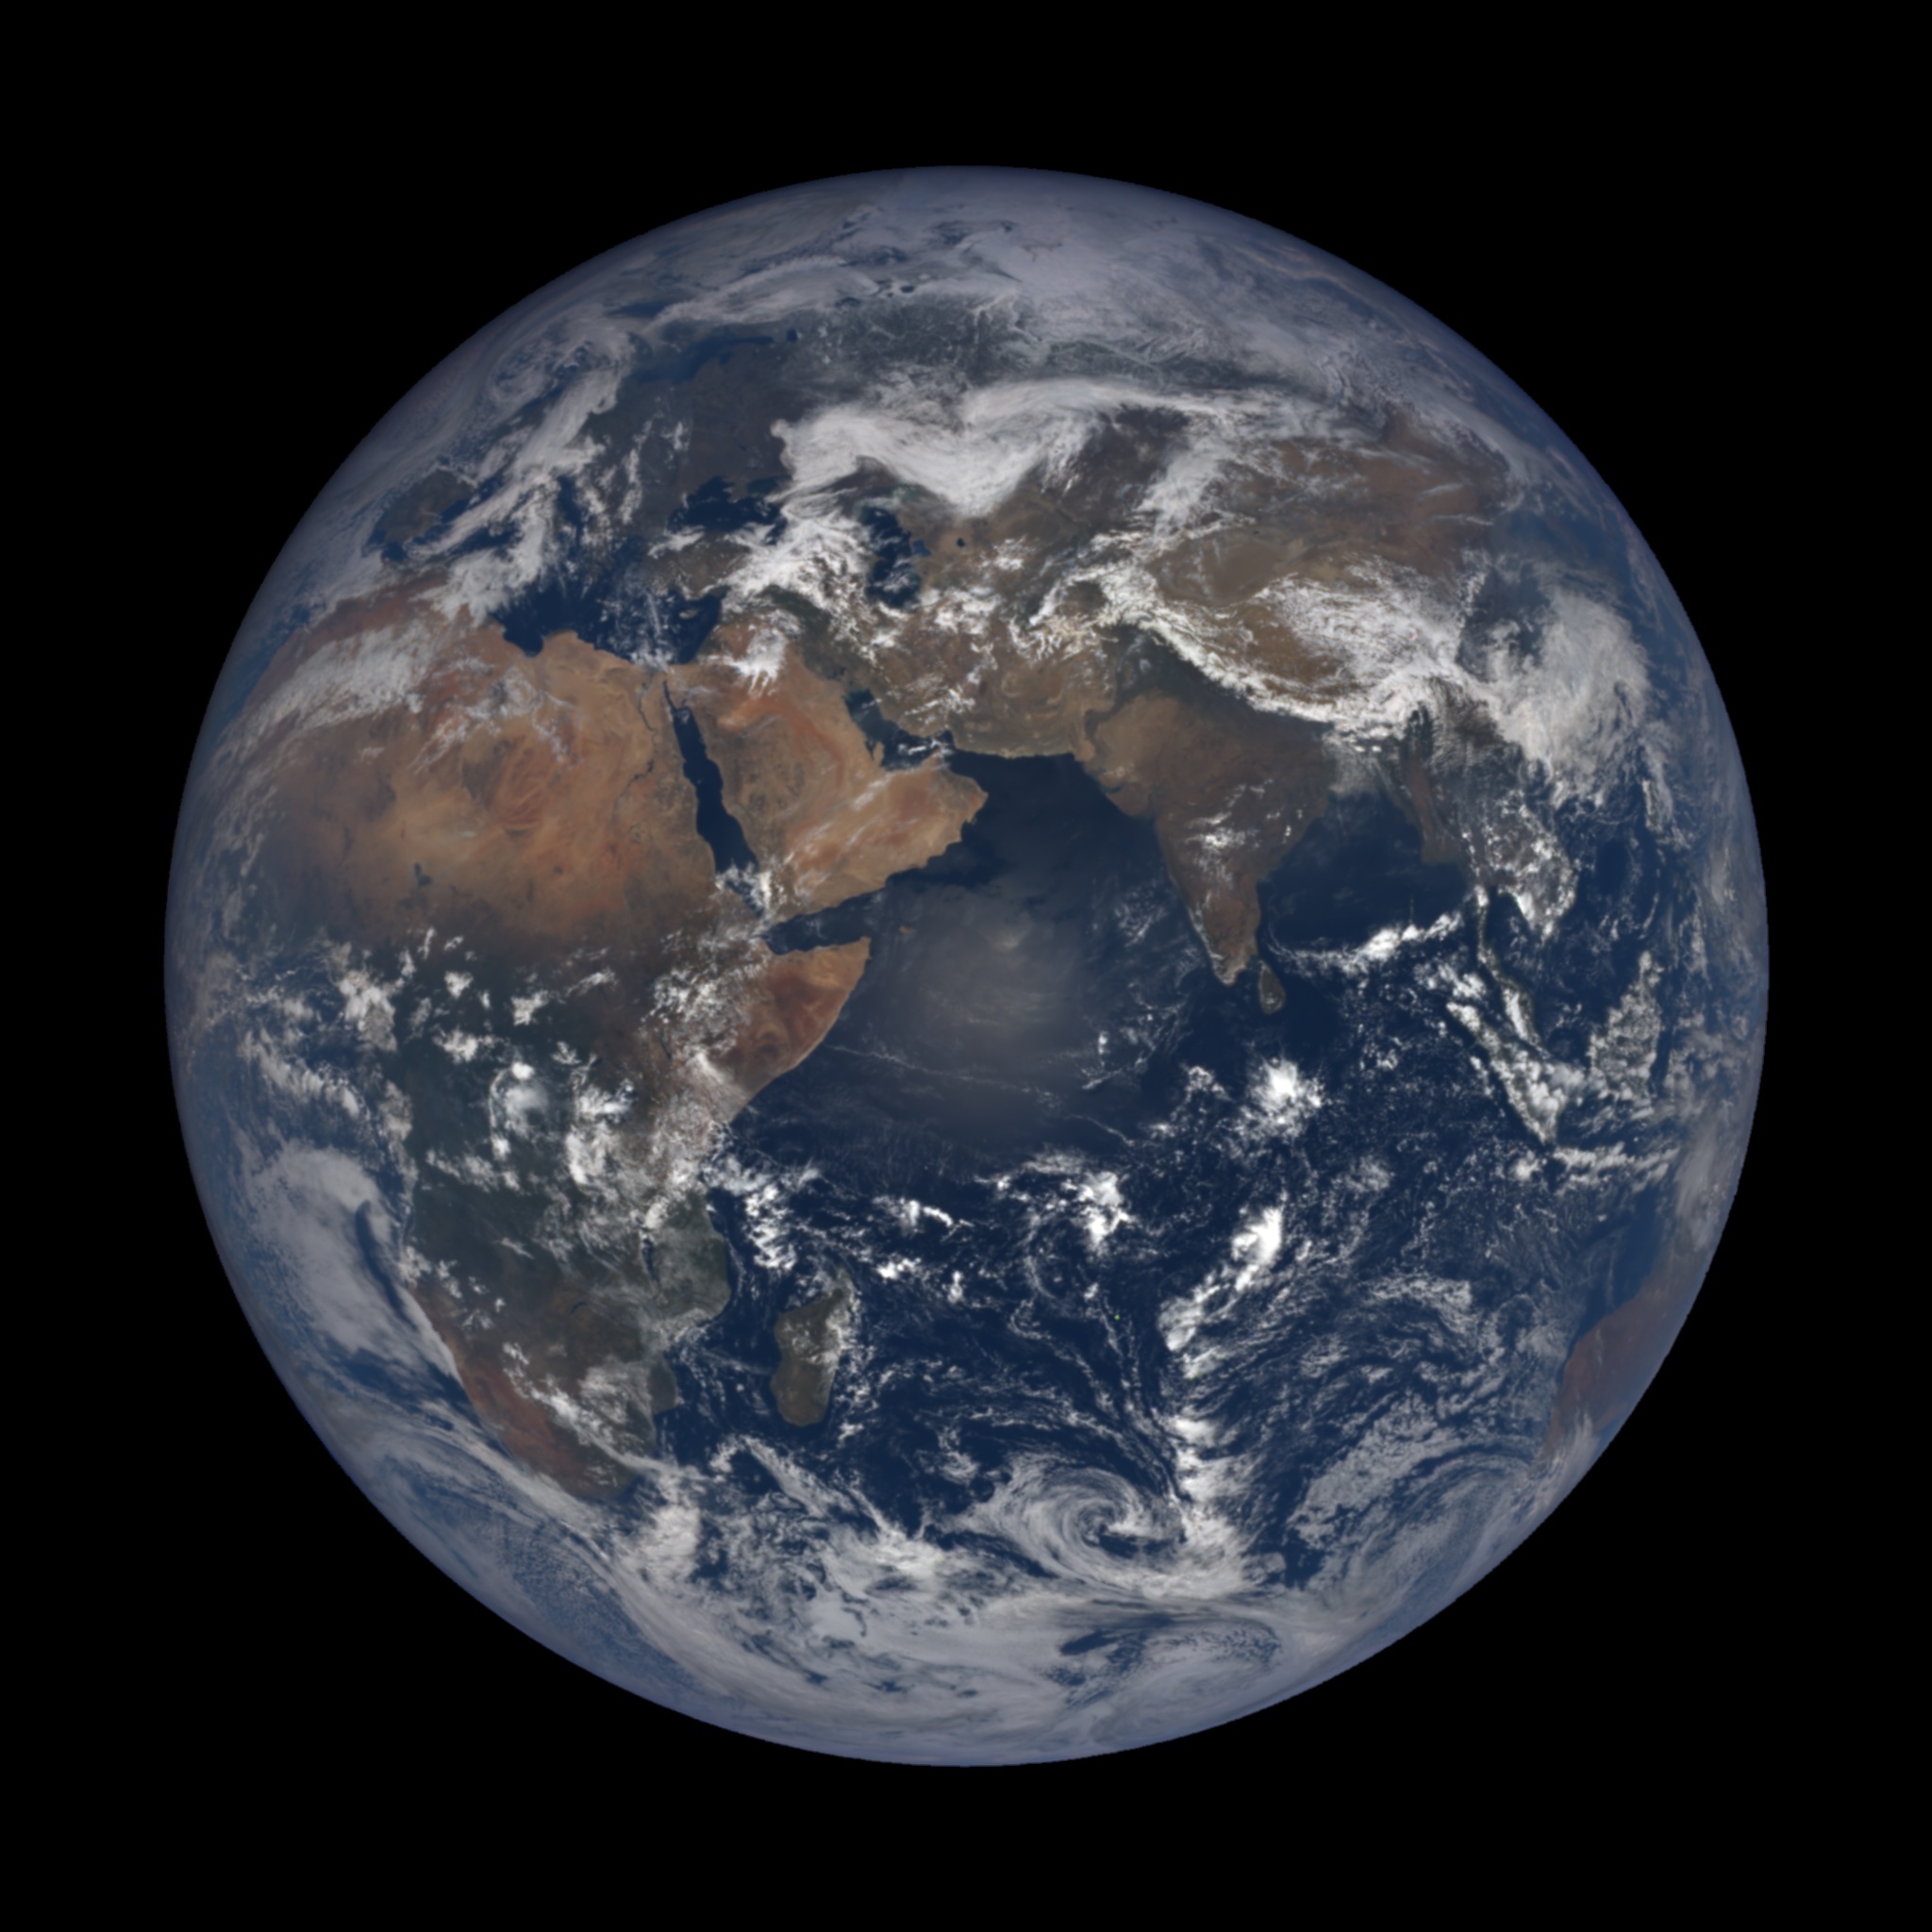
\includegraphics[width=5cm]{images/epic1}
%			%			\includegraphics[width=7cm]{images/fdl}
%		\end{columns}
%	\end{center}
%	
%	\vfill
%\end{frame}
%}

{\setbeamercolor{background canvas}{bg=tumbluedark}
	\begin{frame}[plain]
	
	\vfill
	\Huge\color{white}
	\begin{center}
		\begin{columns}
			\column{.5\textwidth}
			\vspace{7em}
			
			\hfill 
			Vegetation Modeling
			\column{.5\textwidth}
			
			
\includegraphics[width=\textwidth]{images/Large1954_cerial_growth_stages_white}
			%%			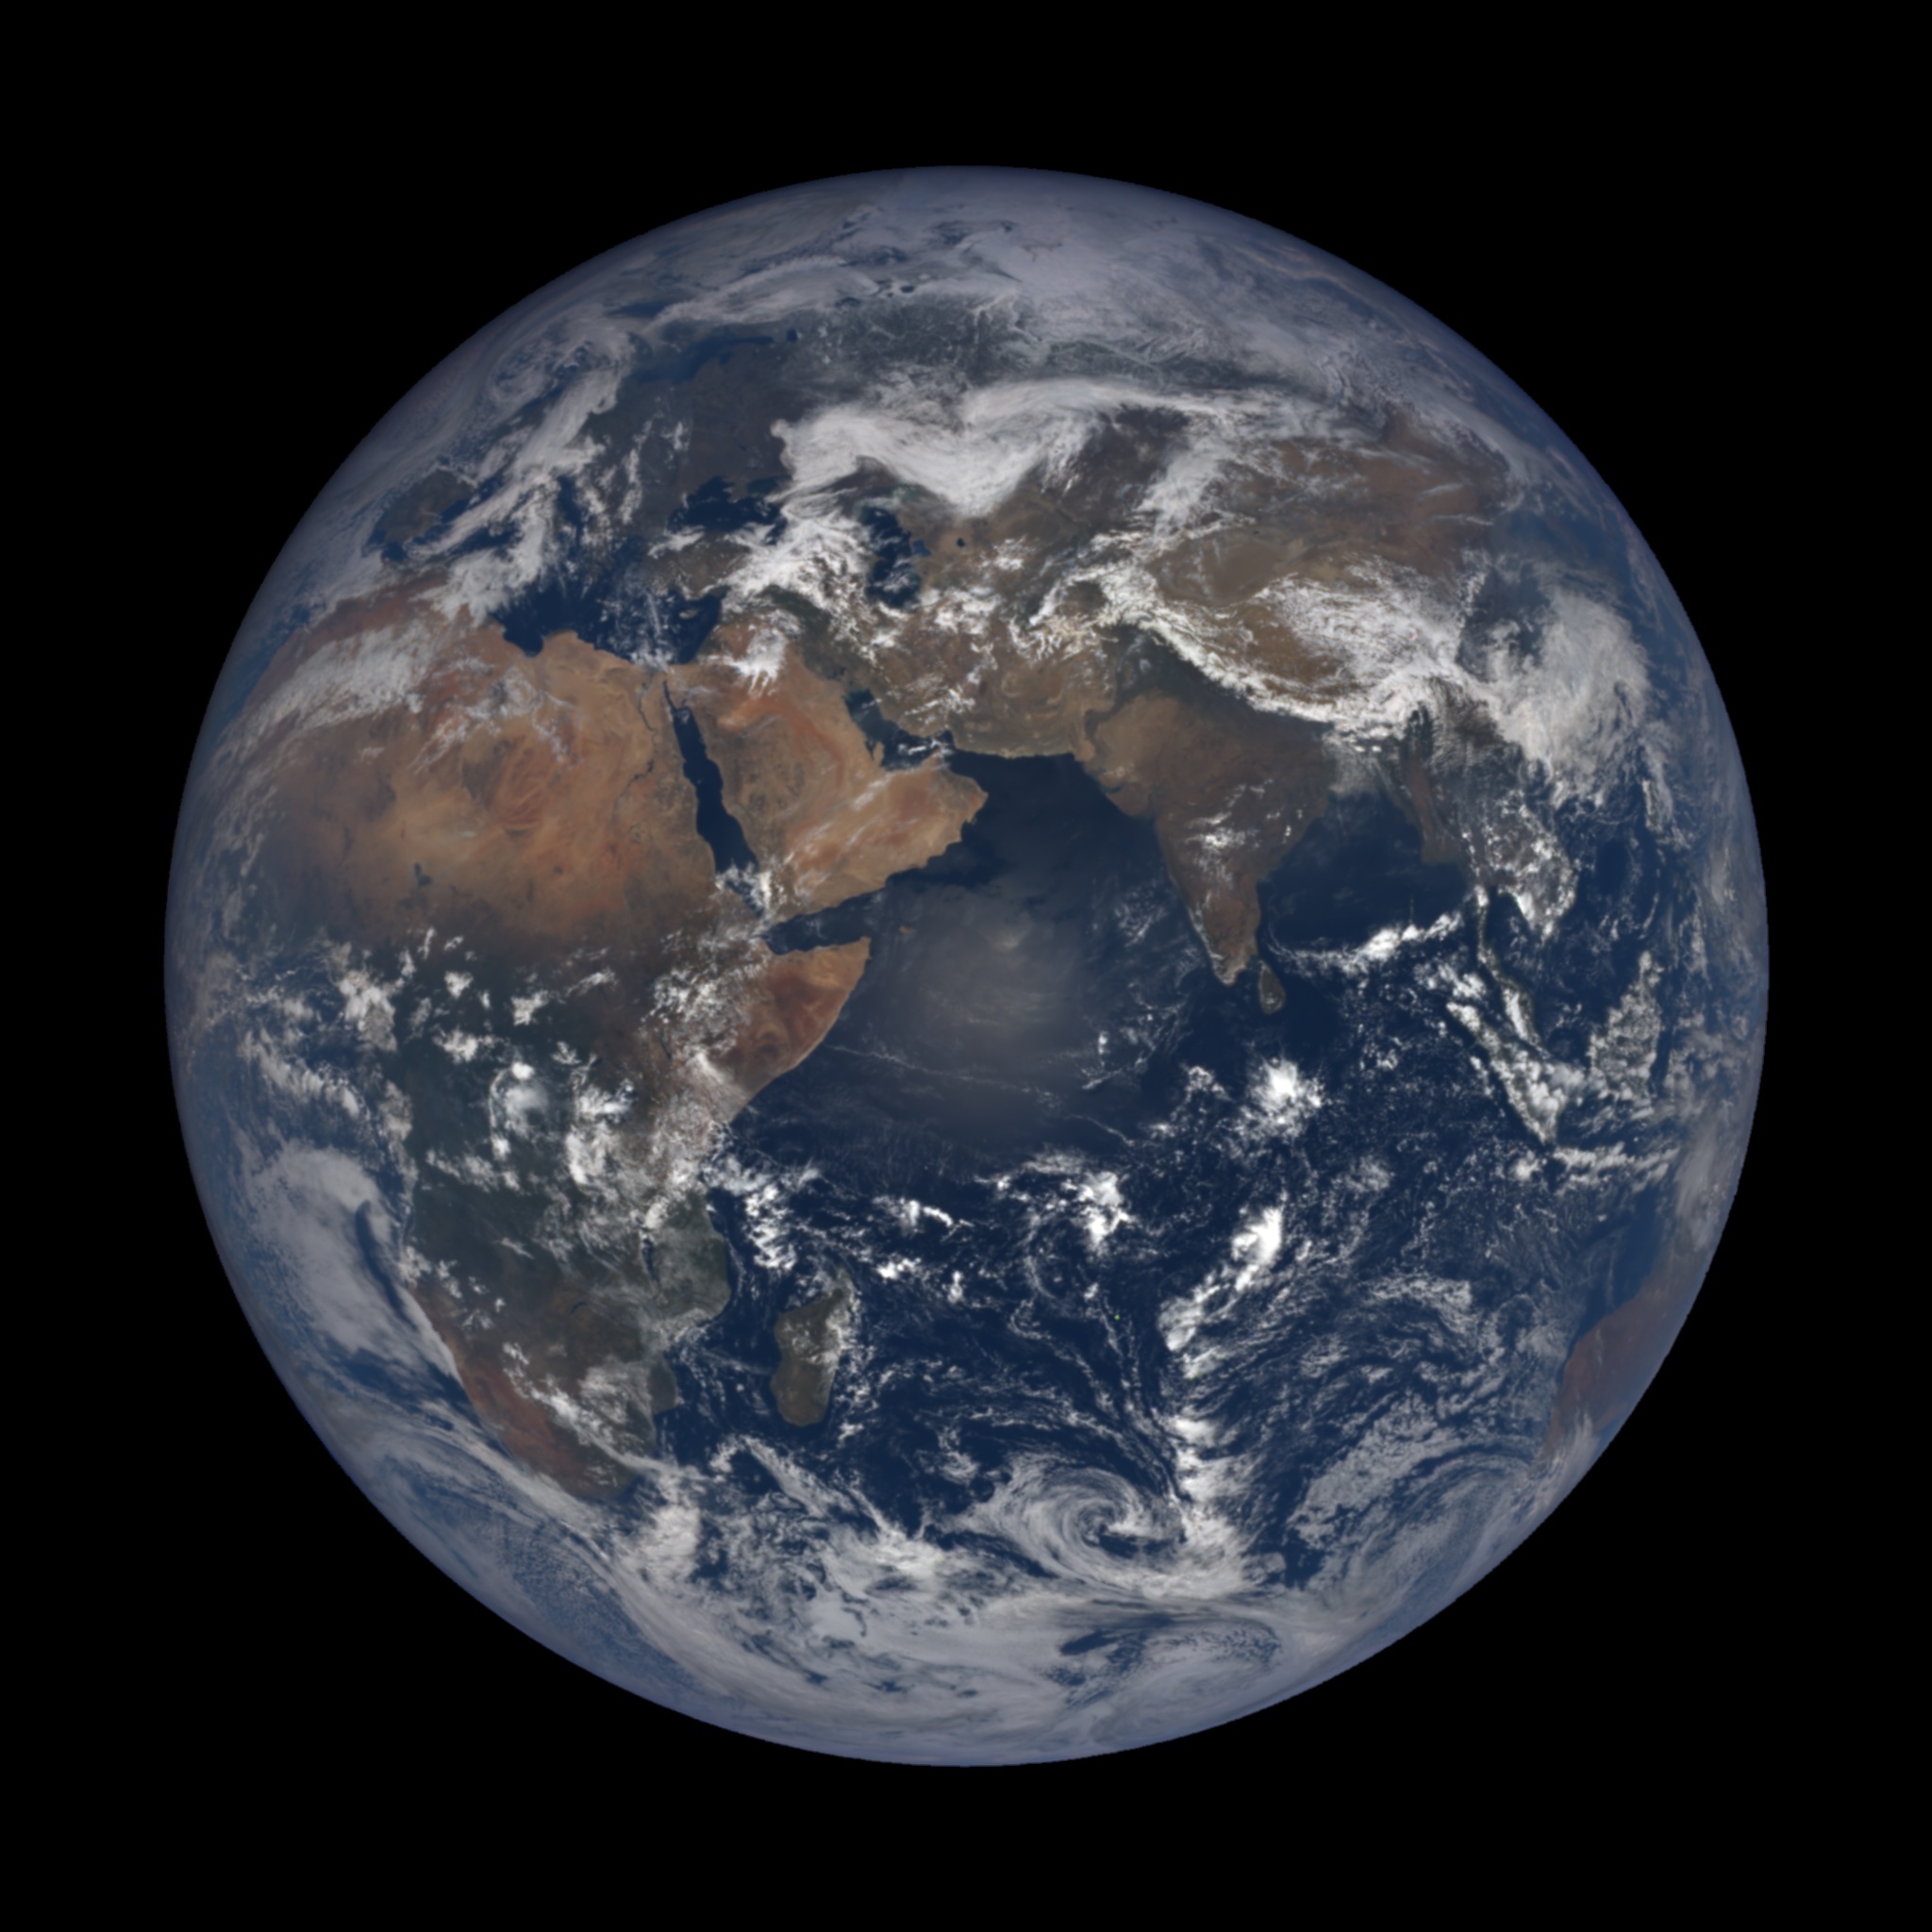
\includegraphics[width=5cm]{images/epic1}
			%			\includegraphics[width=7cm]{images/fdl}
		\end{columns}
		\small\raggedleft(Large et al., 1954)
	\end{center}
	
	\vfill
\end{frame}
}

\newcommand{\rastergrid}{
\begin{tikzpicture}
% each layer
\begin{scope}[scale=2]

% raster size
\def\d{0.7}		

% distance layer
\def\s{\d*5}

\foreach \i in {1,...,6}
{		
\begin{scope}[
yshift=\s*\i,every node/.append style={
	yslant=0.5,xslant=-1},yslant=0.5,xslant=-1
]
%\draw[step=3.33mm] (0,0) grid (1,1);
%\fill[black,fill opacity=.9] (0.333,0.333) rectangle (0.333,0.333);    	    	  

\foreach \row in {0,...,2}{
	\foreach \col in {0,...,2}{
		\draw[tumblack, fill=tumblue!\pdfuniformdeviate 40,fill opacity=1,rounded corners=1] (\col*\d/3,\row*\d/3) rectangle (\col*\d/3+\d/3, \row*\d/3+\d/3);
		%                 \draw[black, fill=black!\pdfuniformdeviate 40,fill opacity=1,rounded corners=1] (\col*\d/3,\row*\d/3) rectangle (\col*\d/3+\d/3, \row*\d/3+\d/3);
	}
}

%\draw[step=3.33mm] (0,0) grid (1,1);
%\fill[white,fill opacity=.9] (0,0) rectangle (1,1);
\end{scope}
}
\end{scope}
\end{tikzpicture}
}


%\begin{frame}
%\frametitle{Spectral Band}
%\end{frame}


\begin{frame}
\frametitle{Multi-temporal Vegetation Modeling}

\begin{columns}
	\column{.5\textwidth}
	
	\begin{tikzpicture}
	\node[] at (0,0){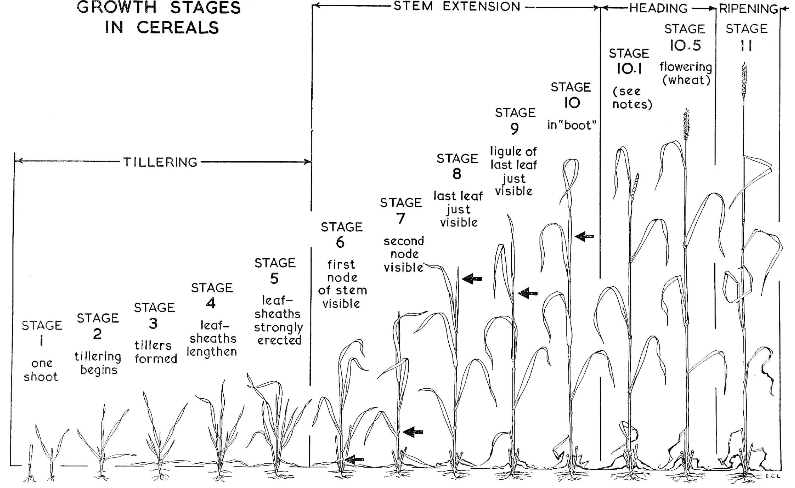
\includegraphics[width=\textwidth]{images/Large1954_cerial_growth_stages}};
	
	%		\draw[step=1.0,black,thin, fill=none] (-2,-2) grid (2,2);
	
	\visible<-1>{\draw [fill=white, draw=none, opacity=0.8] (-0.8,-3) rectangle (2,2.5);}
	\visible<-2>{\draw [fill=white, draw=none, opacity=0.8] (2,-3) rectangle (5,2.5);}
	
	\visible<1>{\node[rotate=190] at (-2.5,1.5){
\includegraphics[width=15mm]{images/icons/sat2}};}
	\visible<2>{\node[rotate=225] at (-2.5,1.5){
\includegraphics[width=15mm]{images/icons/sat2}};}
	\visible<3->{\node[rotate=260] at (-2.5,1.5){
\includegraphics[width=15mm]{images/icons/sat2}};}
	
	
%	\visible<4->{\node at (-1.5,1.4) {
\includegraphics[width=10mm]{images/cloud}};
%	}
	
	\end{tikzpicture}
	
	\column{.5\textwidth}
	
	{\Large
		\only<1>{
			\begin{equation*}
			f_\text{vegetation}(\V{X}_t)
			\end{equation*}
		}
		\only<2>{
			\begin{equation*}
			f_\text{vegetation}(\V{X}_t,\V{X}_{t+1})
			\end{equation*}
		}
		\only<3>{
			\begin{equation*}
			f_\text{vegetation}(\V{X}_t,\V{X}_{t+1},\V{X}_{t+2})
			\end{equation*}
		}
	}
	
	
	\vspace{2em}
	
	
	\visible<1->{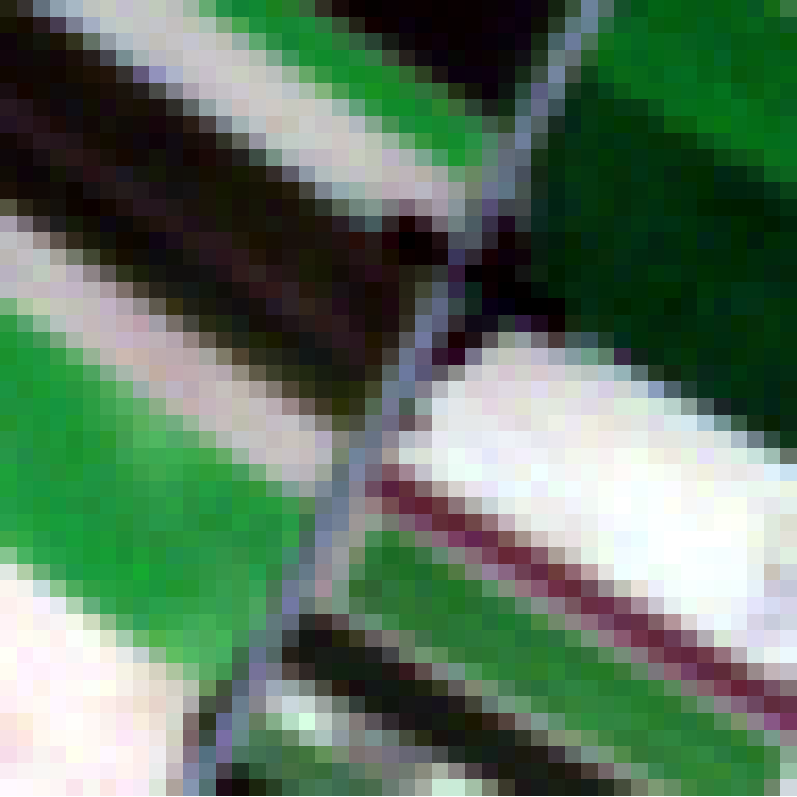
\includegraphics[width=.22\textwidth]{images/s2grid/1}}
	\visible<2->{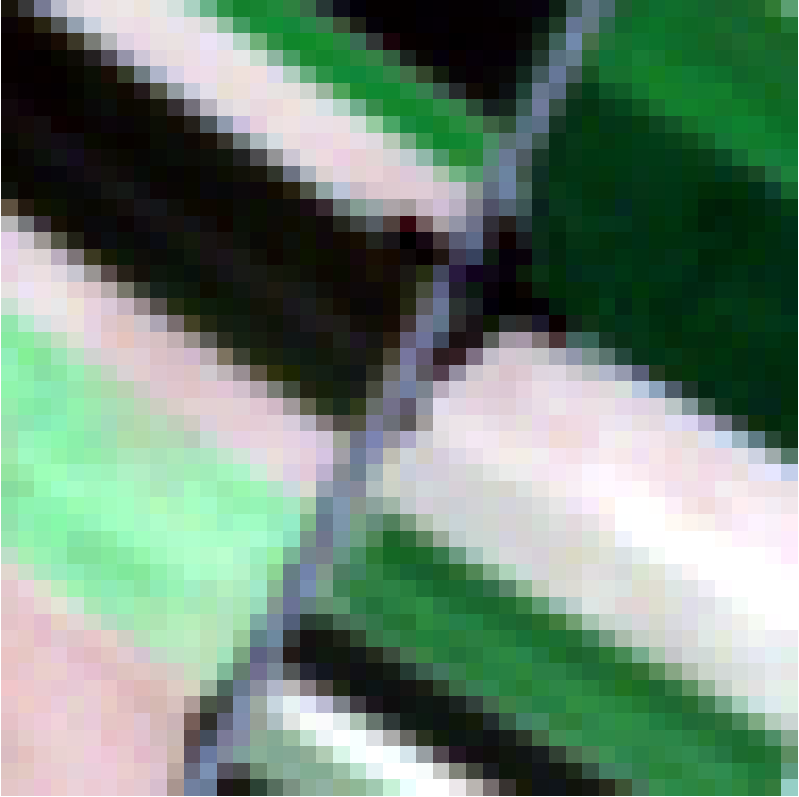
\includegraphics[width=.22\textwidth]{images/s2grid/2}}
	\visible<3->{
\includegraphics[width=.22\textwidth]{images/s2grid/3}}
%	\visible<4->{
\includegraphics[width=.22\textwidth]{images/s2grid/4}}
	
	\vspace{1em}
	
	{\small 
		Large, E. C. (1954). Growth stages in cereals illustration of the Feekes scale. Plant pathology, 3(4), 128-129.
	}
	
	
\end{columns}
\end{frame}

\begin{frame}
	\frametitle{Problem Definition}
	\Large
	
	
	\centering\begin{tikzpicture}[node distance=0em]
		\visible<2->{\node(y){\V{y}};}
		\visible<2->{\node[right=of y](equals){$=$};}
		\node[right=of equals](f){$f_\text{vegetation}$};
		\visible<1->{\node[right=of f](x){$(\V{X}_t,\V{X}_{t+1},\V{X}_{t+2})$};}
		
		\end{tikzpicture}
	
	\vspace{1em}
	\raggedright
	
	\begin{description}\setlength\itemsep{1em}
		\item[\color{tumblue}Problem:]<1-> \textbf{unsupervised learning} of a vegetation model \textbf{is difficult}
		\item[\color{tumblue}Solution:]<2-> re-framing as \textbf{supervised classification} of crop type labels
		\item[\color{tumblue}Intuition:]<3-> A \textbf{supervised classification model} must \textbf{internalize} a learned \textbf{discriminative model} for the \textbf{vegetation}
	\end{description}
	
\end{frame}

%\tikzsetnextfilename{input}

\newcommand{\timeseries}[1]{
\begin{tikzpicture}[baseline=-.25em]
	
	\tikzstyle{annot} = [font=\small\sffamily, text=tumblue]
	\tikzstyle{point} = [thin, tumbluelight, shorten >= .25em, shorten <= .25em]
	
	% from /home/marc/projects/EV2019/images/example/tstop.txt
%	\def\tstopv{0.6285714285714286}
	\def\class{winter barley}
	
	\begin{groupplot}[
	group style={
		group name=my plots,
		group size=1 by 1,
		columns=1,
		xlabels at=edge bottom,
		xticklabels at=edge bottom,
		vertical sep=1em,
	},
	ylabel near ticks,
	ylabel style={font=\sffamily\small, rotate=-90},
	width=.75\textwidth,
	height=3.8cm,
	axis x line=bottom,
	axis y line=left,
	enlarge x limits=0.01,
	xtick={0,0.25,0.5,0.75,1},
	xticklabels={Januar,April,Juni,September,Dezember},
	ymajorgrids,
	ymin=0, ymax=1.4
	]
	
	
	
	\nextgroupplot[
		no marks,  
		ylabel={},
		draw opacity=.8,
		smooth=0.01,
		legend columns=2,
		legend style={at={(.5,1.1)},anchor=south, line width=1pt, fill=tumblue!10}
		]
		 
	\addplot[b1color] table [x=t, y=B1, col sep=comma, forget plot] {images/example/#1};
	\addplot[b9color] table [x=t, y=B9, col sep=comma, forget plot] {images/example/#1};
	\addplot[b10color] table [x=t, y=B10, col sep=comma] {images/example/input.csv};
	
	\addplot[b11color] table [x=t, y=B11, col sep=comma, forget plot] {images/example/#1};
	\addplot[b12color] table [x=t, y=B12, col sep=comma] {images/example/#1};
	
	\addplot[b5color] table [x=t, y=B5, col sep=comma, forget plot] {images/example/#1};
	\addplot[b6color] table [x=t, y=B6, col sep=comma, forget plot] {images/example/#1};
	\addplot[b7color] table [x=t, y=B7, col sep=comma, forget plot] {images/example/#1};
	\addplot[b8color] table [x=t, y=B8, col sep=comma, forget plot] {images/example/#1};
	\addplot[b8Acolor] table [x=t, y=B8A, col sep=comma] {images/example/#1};
		
	\addplot[b2color] table [x=t, y=B2, col sep=comma, forget plot] {images/example/#1};
	\addplot[b3color] table [x=t, y=B3, col sep=comma, forget plot] {images/example/#1};
	\addplot[b4color] table [x=t, y=B4, col sep=comma] {images/example/#1};
%	
	\legend{3 atmospheric, 2 short-wave infrared, 5 near infrared, 3 visible bands}
	
%	\addplot[thick,colorclassone, name path=y1] table[x=t, y=y1]{\mydata};
%	\addplot[thick,colorclasstwo, name path=y2] table[x=t, y=y2]{\mydata};
%	\addplot[thick,colorclassthree, name path=y3] table[x=t, y=y3]{\mydata};
%	\addplot[thick,colorclassfour, name path=y4] table[x=t, y=y4]{\mydata};
	%\addplot[colorblue!20] fill between[of = y1 and axis];
	%\addplot[colorhgray!20] fill between[of = y2 and axis];
	%\addplot[colorgreen!20] fill between[of = y3 and axis];
	%\addplot[colororange!20] fill between[of = y4 and axis];
	
	
	\end{groupplot}
	
	\end{tikzpicture}
}

\begin{frame}
	\frametitle{Crop Type Labels in Europe}
	
	\begin{columns}
		
	\column{.5\textwidth}
	
	\Large
	
	\begin{description}\setlength\itemsep{1em}
		\item[\color{tumblue}collected] yearly within European \textbf{Common Agricultural Policy} (CAP)
		\item[\color{tumblue}declared] by Farmers at \textbf{crop subsidy} applications
		\item[\color{tumblue}today] slowly made publicly available (on a national basis)
		\item[\color{tumblue}in future] further harmonized within \textbf{Europe's INSPIRE} directive
	\end{description}
	
	\column{.5\textwidth}
	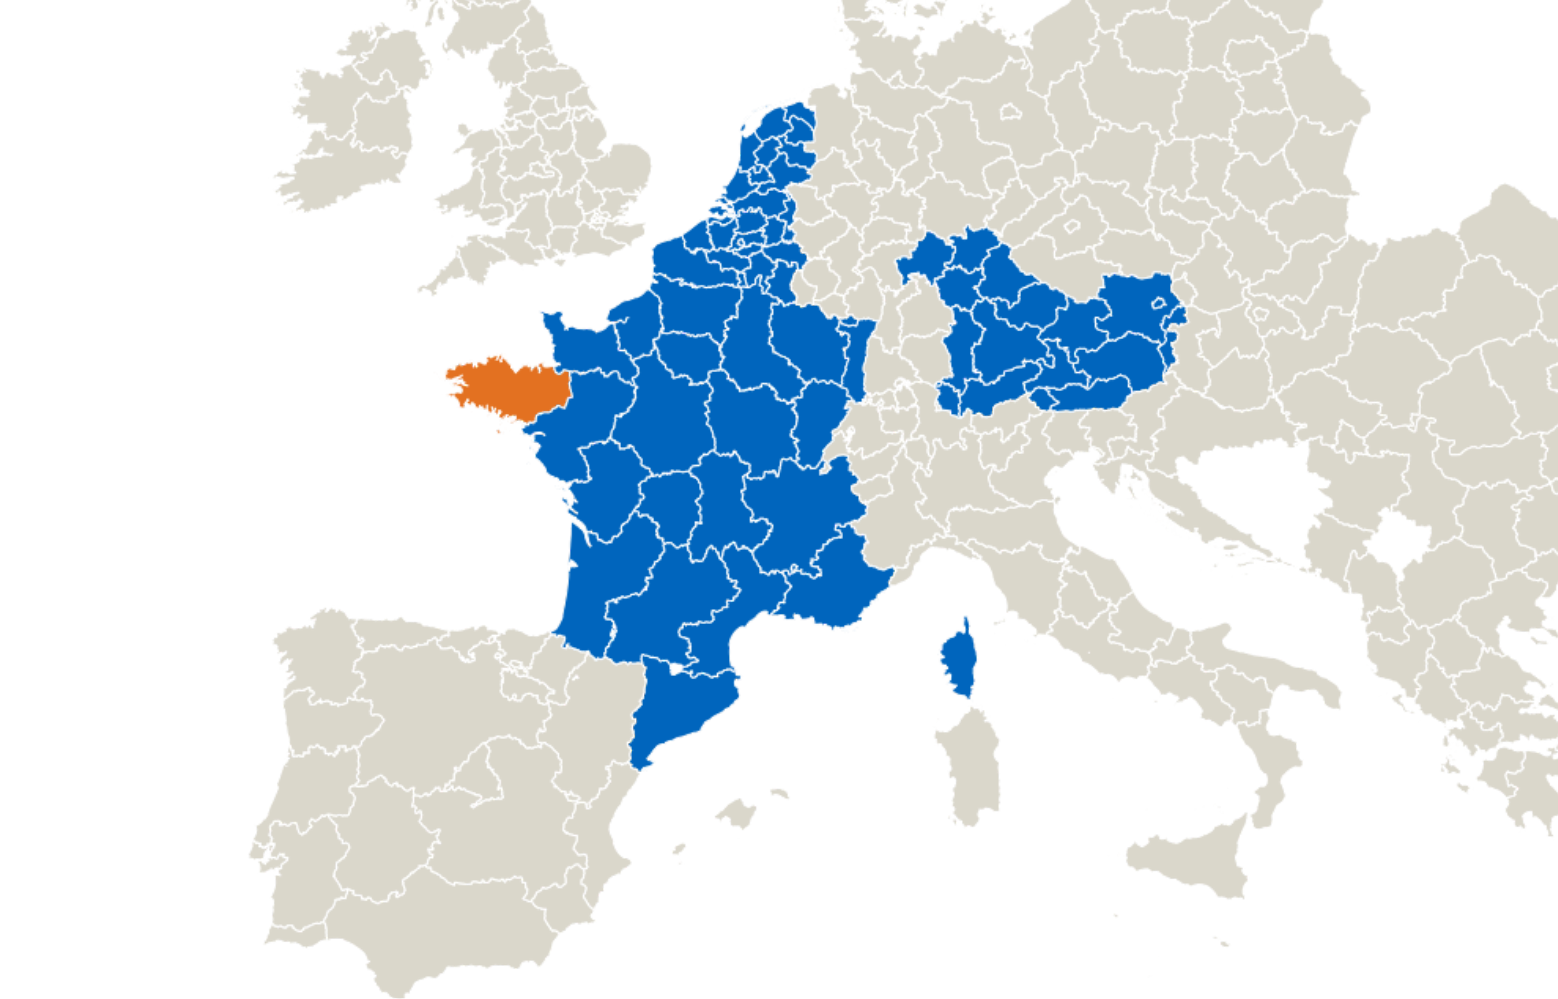
\includegraphics[width=\textwidth]{images/europe_data2}
	
	
	\end{columns}
\end{frame}

{\setbeamercolor{background canvas}{bg=tumbluedark}
	\begin{frame}[plain]
	
	\vfill
	\Huge\color{white}
	\begin{center}
		\begin{columns}
			\column{.5\textwidth}
			\vspace{7em}
			
			\hfill 
			The Dataset
			\column{.5\textwidth}
			
			
\includegraphics[width=\textwidth]{images/map/breizh_white}
			%%			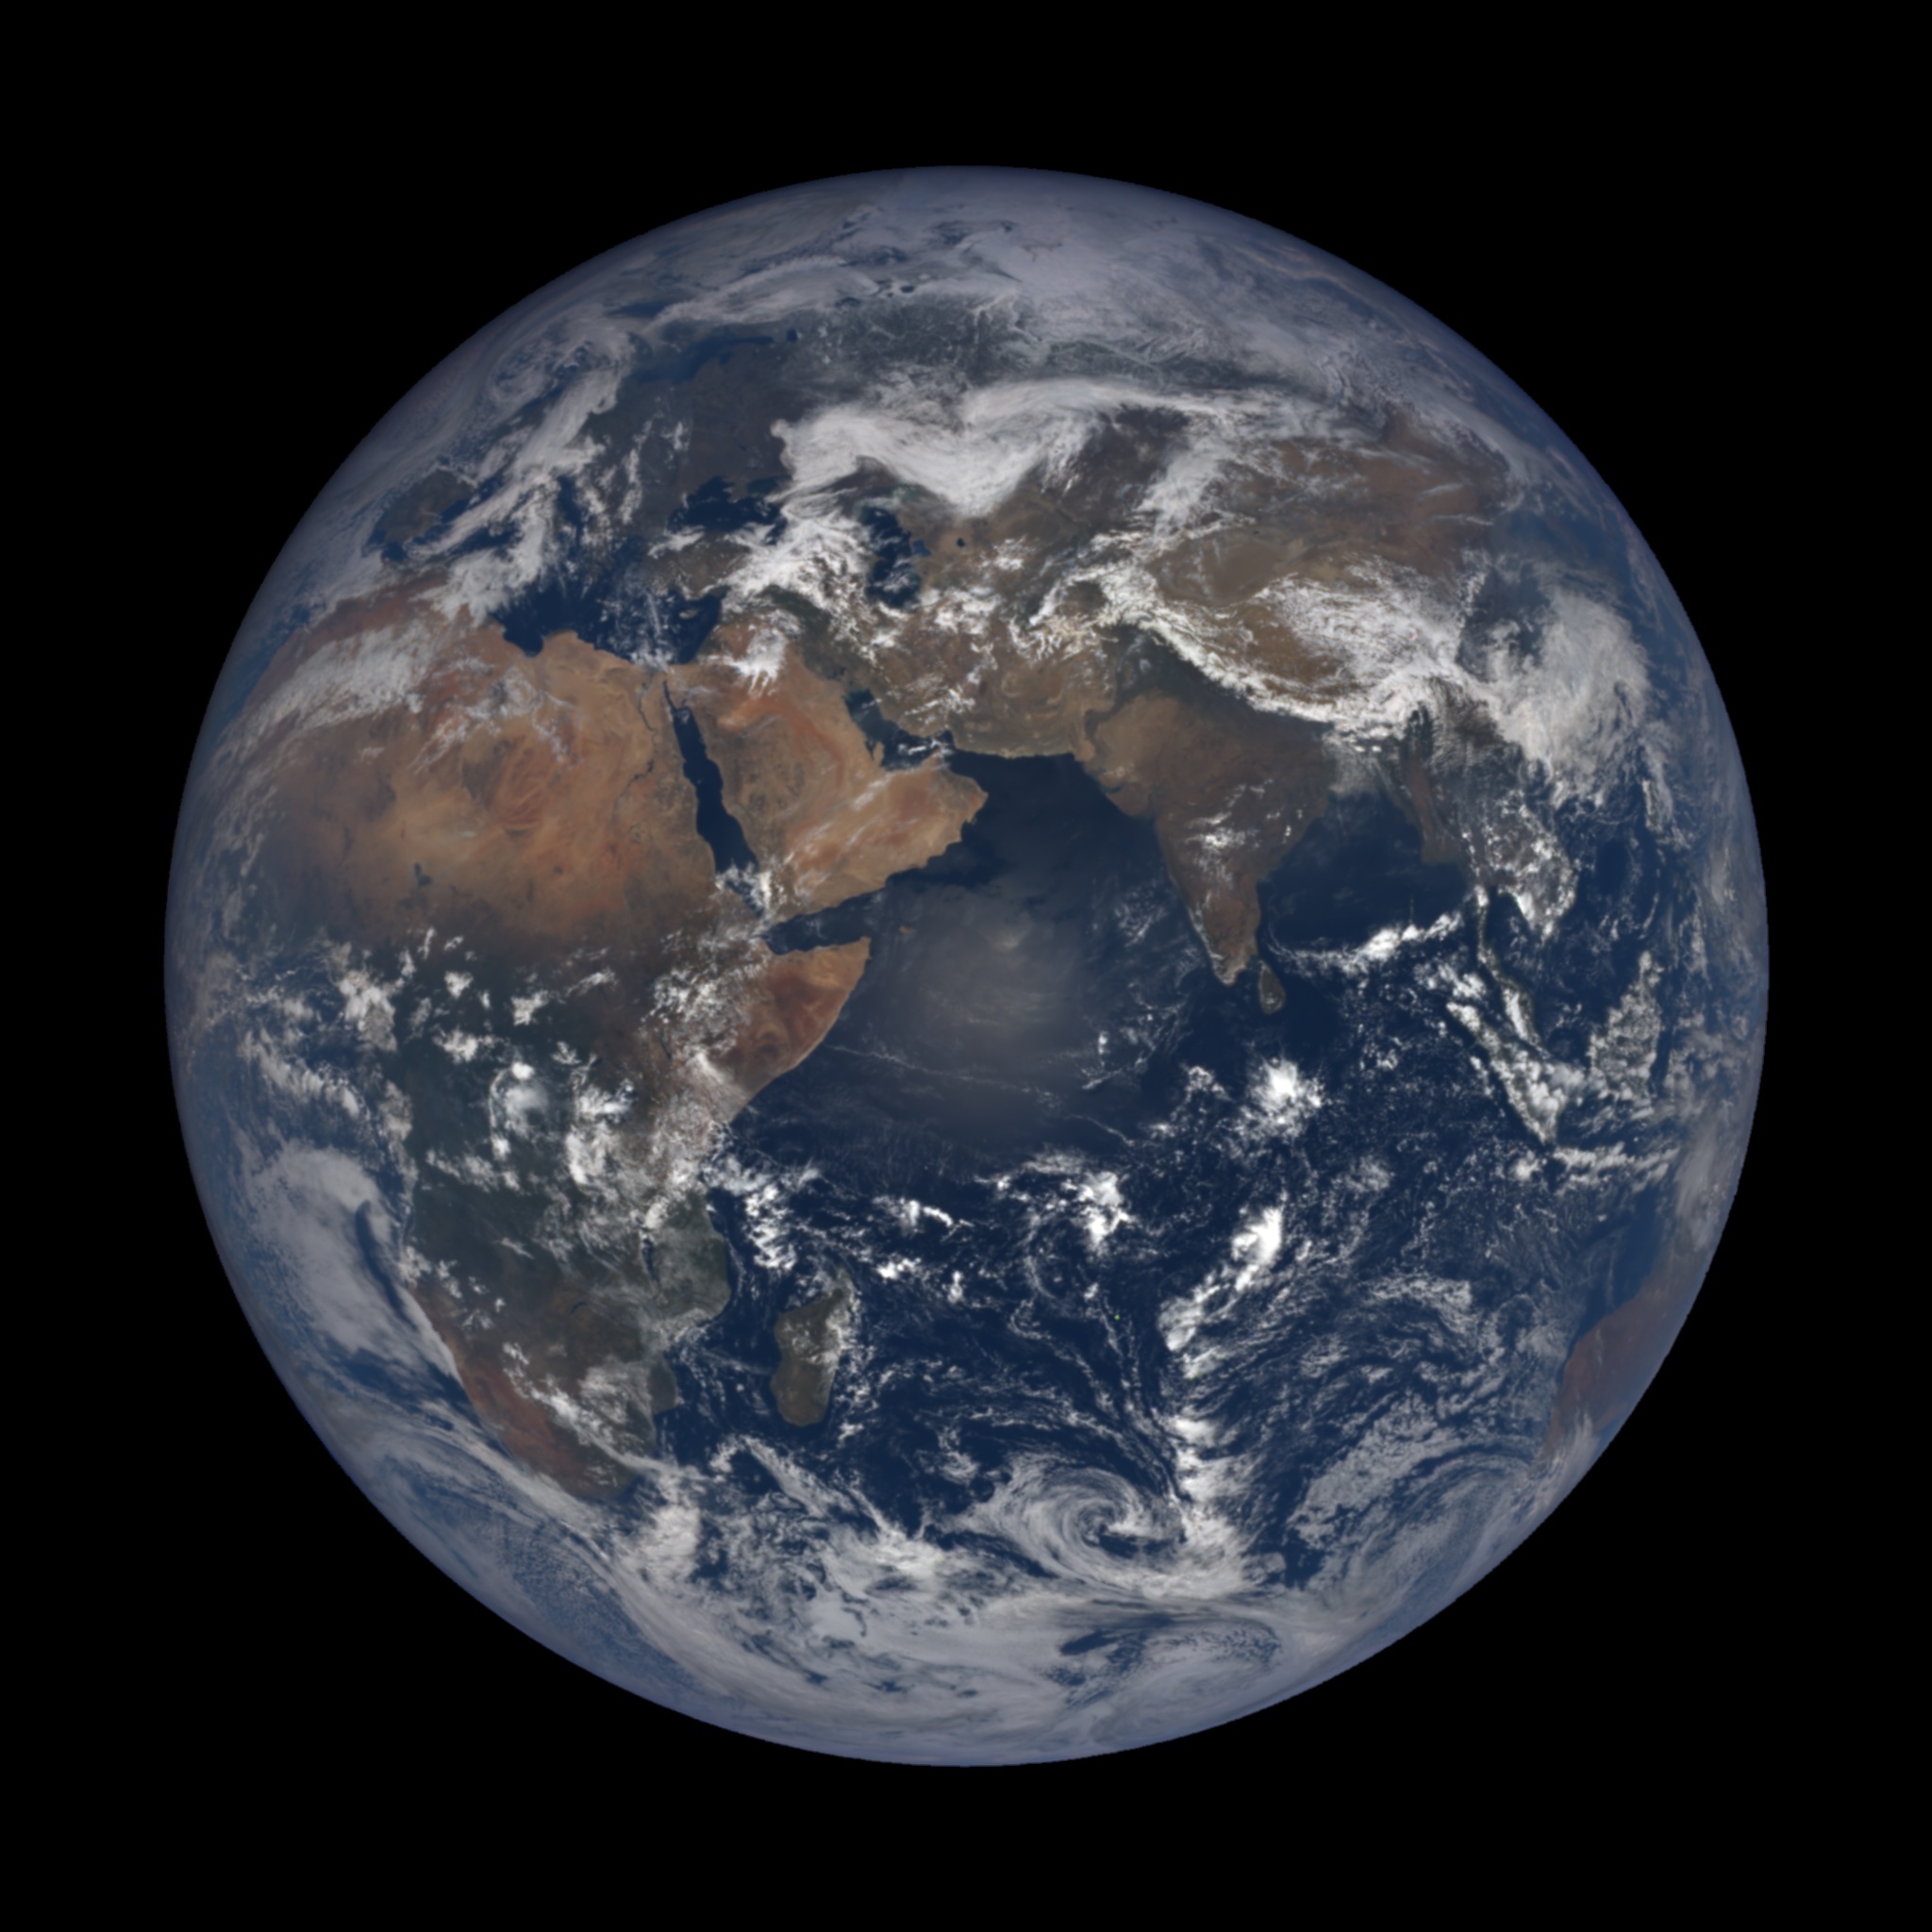
\includegraphics[width=5cm]{images/epic1}
			%			\includegraphics[width=7cm]{images/fdl}
		\end{columns}
		\small\raggedleft Field Parcel Coverage in Brittany
	\end{center}
	
	\vfill
\end{frame}
}

\begin{frame}
	\frametitle{Organization}
	
	\begin{columns}
		\column{.5\textwidth}
			\only<1>{
			
		
		\emph{Nomenclature des unités territoriales statistiques (NUTS)} as European standard of administrative Boundaries. 
		\begin{description}
			\item[NUTS-0] countries
			\item[NUTS-1] states
			\item[NUTS-2] districts
			\item[NUTS-3] municipalities
		\end{description}%NUTS-0 countries, NUTS-1 states, NUTS-2 districts, NUTS-3 municipalities. Add-on: All European Statistics (Eurostats) are collected in these administrative divisions.
		
			}
			\only<2>{
				Field Parcels
				\begin{tabular}{lrrr}
				\toprule
				Departements & NUTS-3 & Parcels & Size \\
				\cmidrule(lr){1-1}\cmidrule(lr){2-2}\cmidrule(lr){3-3}\cmidrule(lr){4-4}
				%			\midrule
				\color{frh04color}\textbf{Morbihan} & FRH04 & 158522 & 4.3 Gb\\
				\color{tumgraydark}\textbf{Côtes-d’Armor} & FRH01 & 221095  & 6.7 Gb \\
				\color{frh02color}\textbf{Finistère} & FRH02 & 180565 & 6.2 Gb \\
				\color{frh03color}\textbf{Ille-et-Vilaine} & FRH03 & 207993 & 6.8 Gb\\
				\\
				\midrule
				Brittany & FRH0 & 768175\\
				\bottomrule
			\end{tabular}
			}
			\vspace{1em}
			
			we suggest a spatially distinct train/test split via these partitions. \\
			\vspace{1em}
			\textbf{Bonus:} Eurostat statistics are gathered on NUTS boundaries. 
		
		\column{.5\textwidth}
			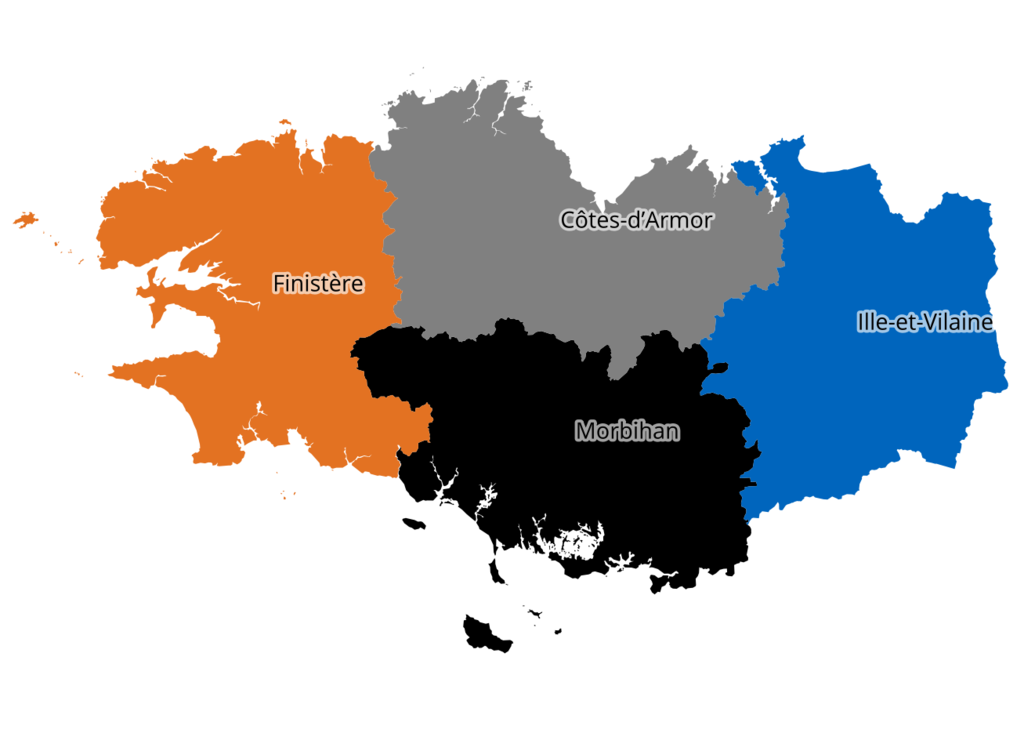
\includegraphics[width=.9\textwidth]{images/map/regions}
			NUTS-3 regions within Brittany, France
		
	\end{columns}
	
\end{frame}


\tikzsetnextfilename{example}

%\newcommand{\wv}[2]{$\lambda_\text{#1}=#2$}
\newcommand{\wv}[2]{$\rho_\text{#2}$}


\newcommand{\examplemeadows}{

\begin{tikzpicture}


\tikzstyle{annot} = [font=\tiny\sffamily, text=tumblue]
\tikzstyle{point} = [thin, tumbluelight, shorten >= .25em, shorten <= .25em]

% from /home/marc/projects/EV2019/images/example/tstop.txt
\def\tstopv{0.6285714285714286}
\def\class{winter barley}

\begin{axis}[date coordinates in=x,
date ZERO=2017-01-01,
xmin=2017-01-01,
xmax=2017-12-31,
ylabel near ticks,
ylabel style={font=\sffamily\small, rotate=0, yshift=-.5em},
width=.95\linewidth,
height=5cm,
axis x line=bottom,
axis y line=left,
%	enlarge x limits=0.01,
xtick={2017-01-01,2017-05-01,2017-08-01,2017-12-01},
xticklabels={January,April,August,December},
ymajorgrids,
ymax=10000,
thin,
smooth,
no marks,  
ylabel={$\rho \times 10^4$},
draw opacity=.8,
%		tension=0.001,
legend columns=8,
%y tick label style={rotate=90},
%legend to name=leg,
legend style={at={(.5,1.1)},anchor=south, line width=1pt, fill=tumblue!10}
]

%\addlegendimage{empty legend}


\addplot[b1color] table [x=doa, y=B1, col sep=comma] {images/example/3685593.csv};
\addplot[b2color] table [x=doa, y=B2, col sep=comma] {images/example/3685593.csv};
\addplot[b3color] table [x=doa, y=B3, col sep=comma] {images/example/3685593.csv};
\addplot[b4color] table [x=doa, y=B4, col sep=comma] {images/example/3685593.csv};
\addplot[b5color] table [x=doa, y=B5, col sep=comma] {images/example/3685593.csv};
\addplot[b6color] table [x=doa, y=B6, col sep=comma] {images/example/3685593.csv};
\addplot[b7color] table [x=doa, y=B7, col sep=comma] {images/example/3685593.csv};
\addplot[b8color] table [x=doa, y=B8, col sep=comma] {images/example/3685593.csv};
\addplot[b8Acolor] table [x=doa, y=B8A, col sep=comma] {images/example/3685593.csv};
\addplot[b9color] table [x=doa, y=B9, col sep=comma] {images/example/3685593.csv};
\addplot[b10color] table [x=doa, y=B10, col sep=comma] {images/example/3685593.csv};
\addplot[b11color] table [x=doa, y=B11, col sep=comma] {images/example/3685593.csv};
\addplot[b12color] table [x=doa, y=B12, col sep=comma] {images/example/3685593.csv};

%\node[above=of leg]{test};
%
%\addlegendentry{$\sqrt{x}$}
%\addlegendentry{$\ln{x}$}
%
%\addlegendentry[xshift=-10pt, font=\bfseries]{S2 Satellite Bands}

\addlegendentry{\wv{B01}{443nm}}
\addlegendentry{\wv{B2}{492nm}}
\addlegendentry{\wv{B3}{560nm}}
\addlegendentry{\wv{B4}{665nm}}
\addlegendentry{\wv{B5}{704nm}}
\addlegendentry{\wv{B6}{740nm}}
\addlegendentry{\wv{B7}{783nm}}
\addlegendentry{\wv{B8}{833nm}}
\addlegendentry{\wv{B8A}{864nm}}
\addlegendentry{\wv{B9}{945nm}}
\addlegendentry{\wv{B10}{1374nm}}
\addlegendentry{\wv{B12}{2202nm}}

%\legend{
%\wv{B01}{443nm},
%\wv{B2}{492nm},
%\wv{B3}{560nm},
%\wv{B4}{665nm},
%\wv{B5}{704nm},
%\wv{B6}{740nm},
%\wv{B7}{783nm},
%\wv{B8}{833nm},
%\wv{B8A}{864nm},
%\wv{B9}{945nm},
%\wv{B10}{1374nm},
%\wv{B11}{1613nm},
%\wv{B12}{2202nm}}


\end{axis}


%\node[font=\scriptsize\sffamily, anchor=west] at (0.2,2.7) {Sentinel 2 Satellite Spectral Bands};


\end{tikzpicture}
}


\newcommand{\examplecorn}{
	
	\begin{tikzpicture}
	
	\tikzstyle{annot} = [font=\tiny\sffamily, text=tumblue]
	\tikzstyle{point} = [thin, tumbluelight, shorten >= .25em, shorten <= .25em]
	
	% from /home/marc/projects/EV2019/images/example/tstop.txt
	\def\tstopv{0.6285714285714286}
	\def\class{winter barley}
	
	\begin{axis}[date coordinates in=x,
	date ZERO=2017-01-01,
	xmin=2017-01-01,
	xmax=2017-12-31,
	ylabel near ticks,
	ylabel style={font=\sffamily\small, rotate=0, yshift=-.5em},
	width=.95\linewidth,
	height=5cm,
	axis x line=bottom,
	axis y line=left,
	%	enlarge x limits=0.01,
	xtick={2017-01-01,2017-05-01,2017-08-01,2017-12-01},
	xticklabels={January,April,August,December},
	ymajorgrids,
	ymax=10000,
	thin,
	smooth,
	no marks,  
	ylabel={$\rho \times 10^4$},
	draw opacity=.8,
	%		tension=0.001,
	legend columns=8,
	%y tick label style={rotate=90},
	legend style={at={(.5,1)},anchor=south, line width=1pt, fill=tumblue!10}
	]
	
	
	\addplot[b1color] table [x=doa, y=B1, col sep=comma] {images/example/6139251.csv};
	\addplot[b9color] table [x=doa, y=B9, col sep=comma] {images/example/6139251.csv};
	\addplot[b10color] table [x=doa, y=B10, col sep=comma] {images/example/6139251.csv};
	
	\addplot[b11color] table [x=doa, y=B11, col sep=comma] {images/example/6139251.csv};
	\addplot[b12color] table [x=doa, y=B12, col sep=comma] {images/example/6139251.csv};
	
	\addplot[b5color] table [x=doa, y=B5, col sep=comma] {images/example/6139251.csv};
	\addplot[b6color] table [x=doa, y=B6, col sep=comma] {images/example/6139251.csv};
	\addplot[b7color] table [x=doa, y=B7, col sep=comma] {images/example/6139251.csv};
	\addplot[b8color] table [x=doa, y=B8, col sep=comma] {images/example/6139251.csv};
	\addplot[b8Acolor] table [x=doa, y=B8A, col sep=comma] {images/example/6139251.csv};
	
	\addplot[b2color] table [x=doa, y=B2, col sep=comma] {images/example/6139251.csv};
	\addplot[b3color] table [x=doa, y=B3, col sep=comma] {images/example/6139251.csv};
	\addplot[b4color] table [x=doa, y=B4, col sep=comma] {images/example/6139251.csv};
	
	\node[font=\sffamily] at (rel axis cs:0.35,0.9)(gr){ground signal};
	\draw (gr) -- (rel axis cs:.26,.3);
	\draw (gr) -- (rel axis cs:.2,.3);
	\draw (gr) -- (rel axis cs:.4,.25);
	
	\node[font=\sffamily] at (rel axis cs:0.8,.93)(cl){cloud noise};
	
	\draw (cl) -- (rel axis cs:.68,.7);
	\draw (cl) -- (rel axis cs:.58,.7);
	\draw (cl) -- (rel axis cs:.81,.7);
	
%	\legend{3 atmospheric, 2 short-wave infrared, 5 near infrared, 3 visible bands}
%	
	
	\addlegendentry{\wv{B01}{443nm}}
	\addlegendentry{\wv{B2}{492nm}}
	\addlegendentry{\wv{B3}{560nm}}
	\addlegendentry{\wv{B4}{665nm}}
	\addlegendentry{\wv{B5}{704nm}}
	\addlegendentry{\wv{B6}{740nm}}
	\addlegendentry{\wv{B7}{783nm}}
	\addlegendentry{\wv{B8}{833nm}}
	\addlegendentry{\wv{B8A}{864nm}}
	\addlegendentry{\wv{B9}{945nm}}
	\addlegendentry{\wv{B10}{1374nm}}
	\addlegendentry{\wv{B12}{2202nm}}
	

	\end{axis}
	
	\end{tikzpicture}
}
\begin{frame}
	\frametitle{Corn Example}
	\examplecorn
\end{frame}

%
%\begin{frame}
%\frametitle{Examples}
%\centering
%%\externalize{beispiel}{%
%\begin{tikzpicture}[node distance=.1em]
%%	\visible<1>{
%%	\node[font=\huge](veg) at (0,0){Vegetationsmodell};
%%	\node[right=0em of veg](input){$\left(\satimage{1},\satimage{1},\satimage{3}\right)$};
%%	}
%\node[font=\huge, label=$f$](equals){$\leftarrow$};
%%	\visible<2>{\node[right=0em of equals](input){\timeseries{input.csv}};}
%\visible<1>{
%	\node[right=0em of equals](input){\timeseries{prep74526670.csv}};}
%
%\visible<2>{\node[right=0em of equals](input){\timeseries{prep77770412.csv}};}
%
%\visible<1>{\node[left= of equals, font=\huge](probas){meadows};}
%\visible<2>{\node[left= of equals, font=\huge](probas){corn};}
%
%
%\end{tikzpicture}%
%%}
%\end{frame}


{\setbeamercolor{background canvas}{bg=tumbluedark}
	\begin{frame}[plain]
	
	\vfill
	\Huge\color{white}
	\begin{center}
		\begin{columns}
			\column{.5\textwidth}
			\vspace{7em}
			
			\hfill 
			Baseline Results
			\column{.5\textwidth}
			
			%			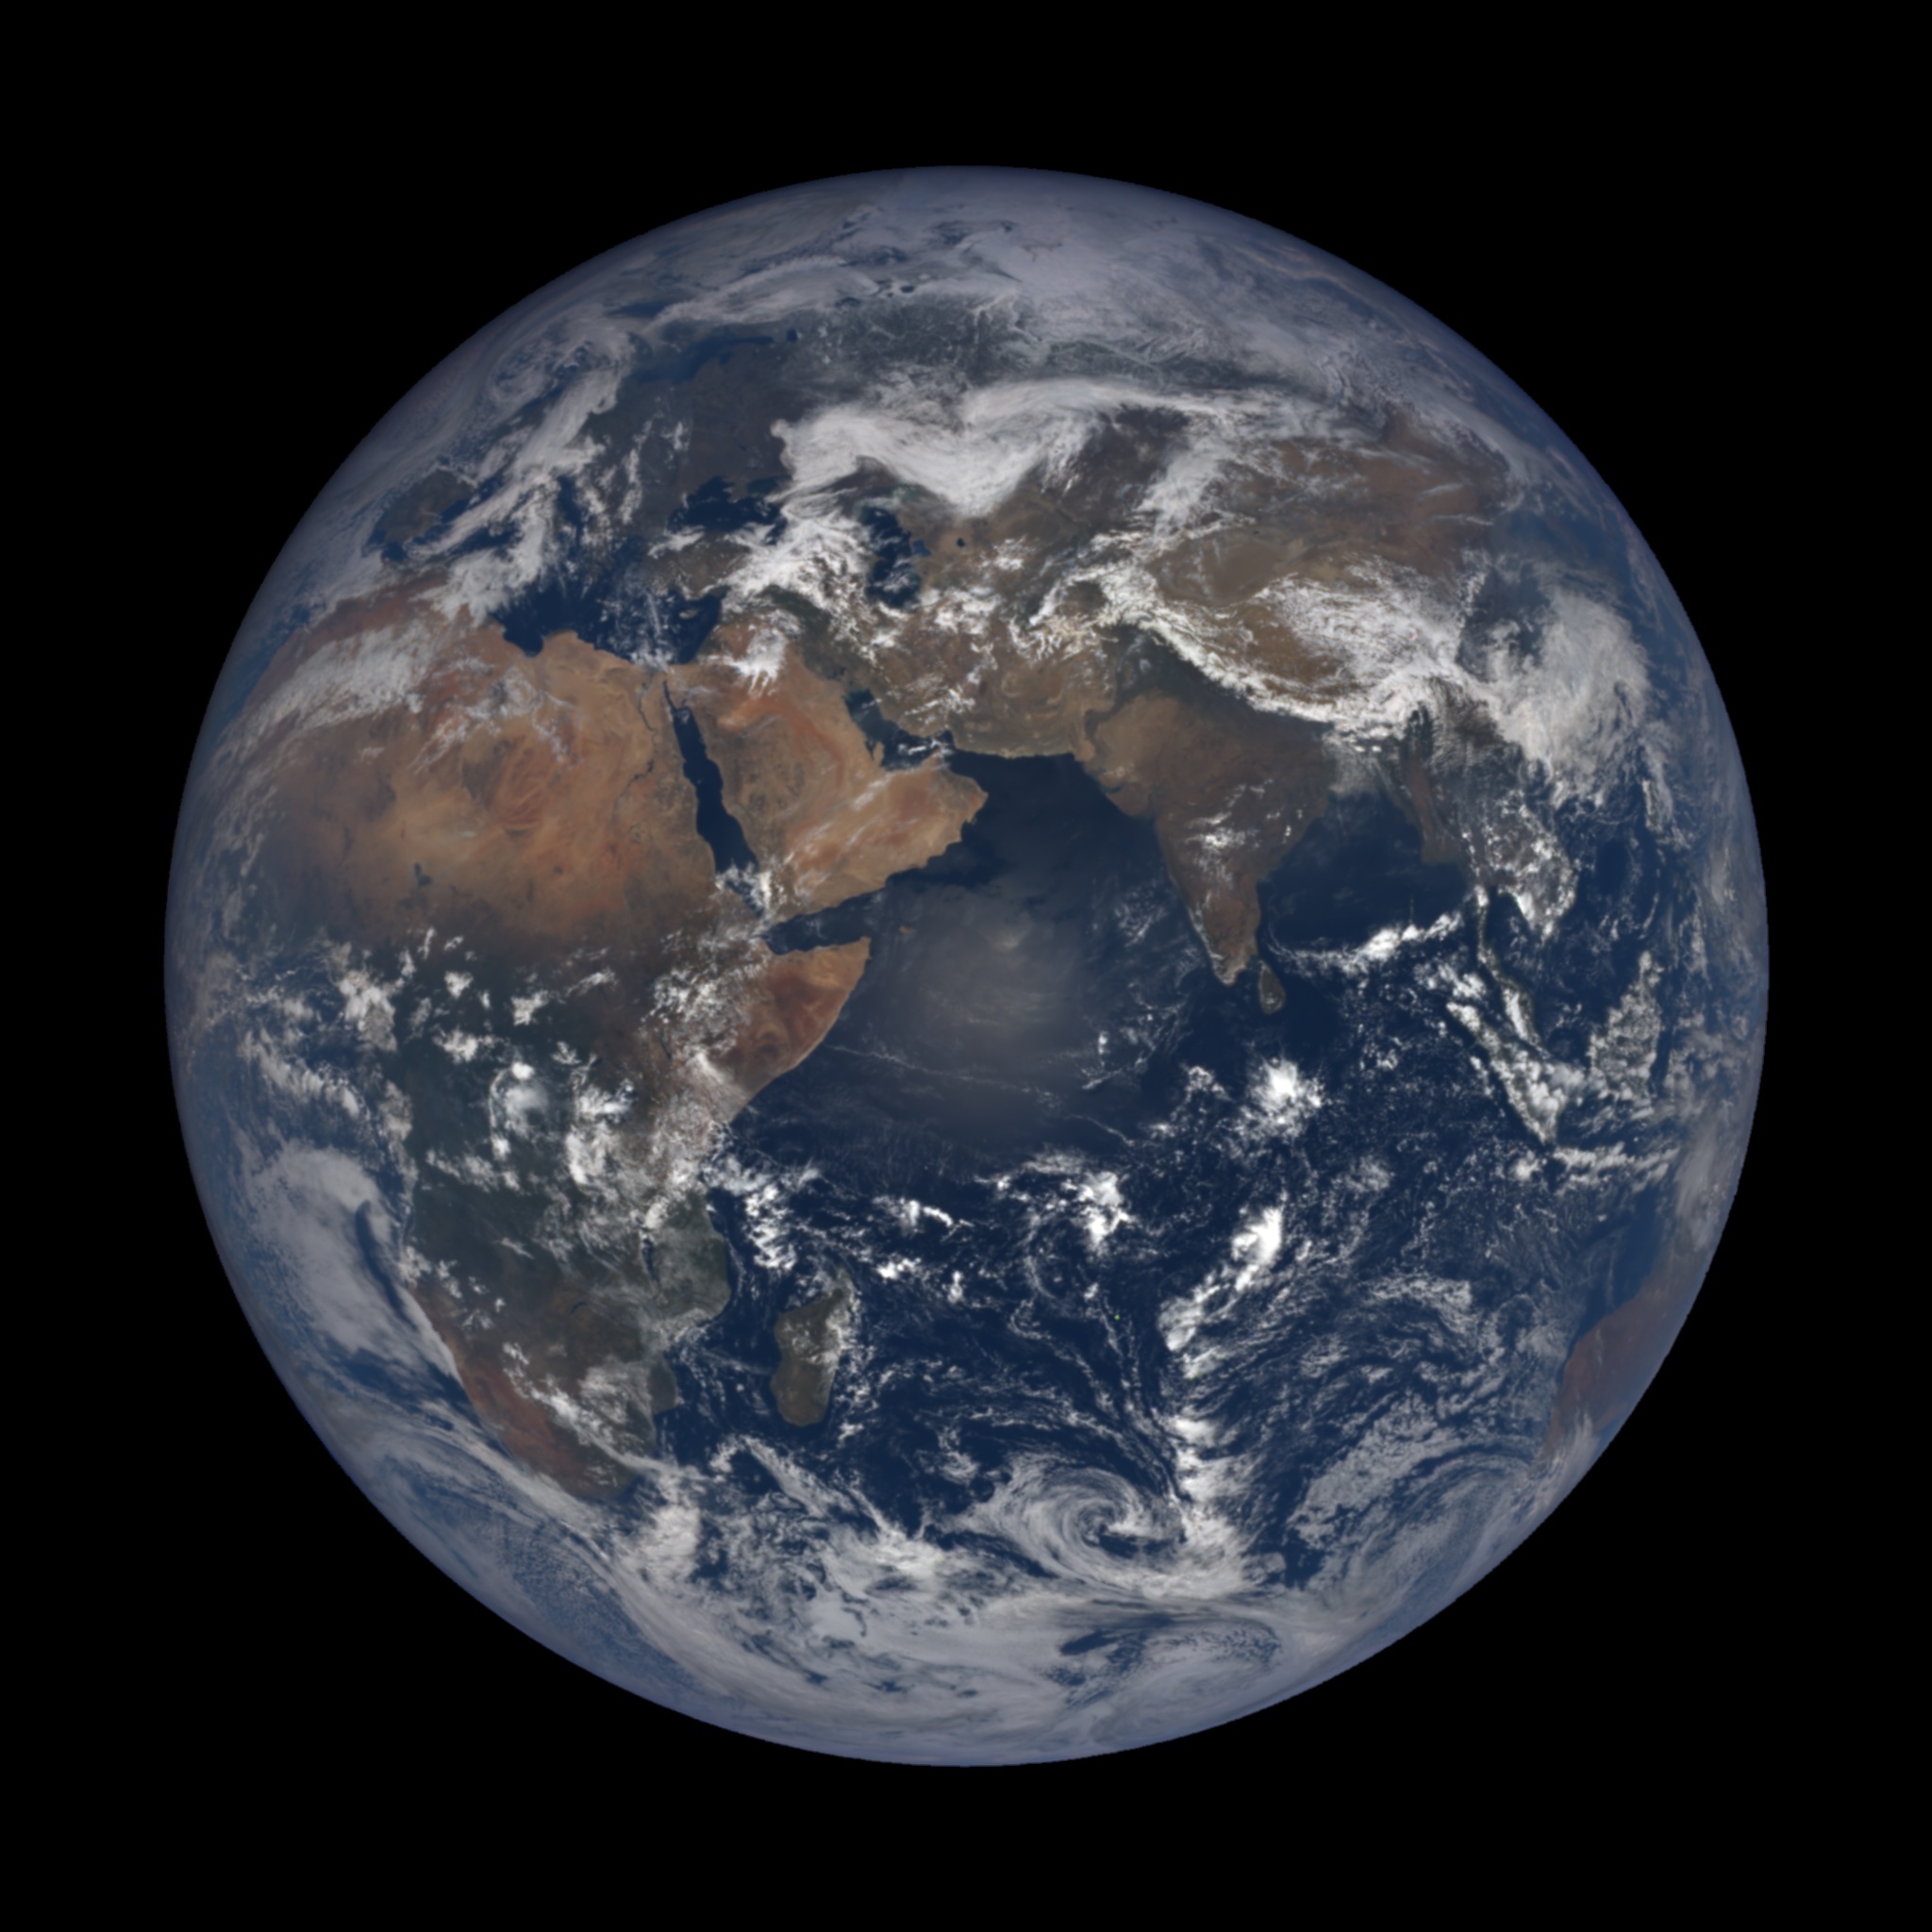
\includegraphics[width=5cm]{images/epic1}
			%\includegraphics[width=7cm]{images/fdl}
		\end{columns}
	\end{center}
	
	\vfill
\end{frame}
}

\newcommand{\confmat}[3]{

\begin{tikzpicture}

  \def\vmax{#3}
  \def\dataindex{#2}
  
%
%  \pgfplotsset{every axis label/.append style={font=\footnotesize},tick pos=right, ylabel near ticks}
%  
%  \pgfplotsset{
%    axis line style={%
%      opacity=0 
%    }   
%  }

  \begin{groupplot}[
  	group style={
  		group size=2 by 1,
  		xlabels at=edge bottom,
  		ylabels at=edge left,
  		xticklabels at=edge bottom,
  		vertical sep=35pt,
  		group name=seq_len_plot
  	},
  	axis line style={draw=none},
  	title style={yshift=.75em,},
    width=6cm,
    height=6cm,
    enlargelimits=false,
    xtick=data,
%     ymin=1,
    xtick distance=1,
    ytick distance=1,
    colormap={example}{%
		color=(tumwhite)%color=(tumbluelight)
%		color=(tumivory)
%		color=(tumorange)
		color=(tumblue)%color=(tumbluelight)
%		color=(tumblack)
	},
    ytick=data,
    ytick align=outside,
    xtick align=outside,
%    tick style={draw=none},
    ytick pos = left,  
    tick label style = {font=\tiny\sansmath\sffamily},
    %xticklabel = {xshift=-0.75cm}
    yticklabel pos=left,
    %yticklabel near ticks,
    xlabel={\normalsize predicted},
    xlabel style={yshift=1em},
    ylabel style={yshift=-3em},
    x label style={at={(axis description cs:0.5,1)},anchor=south},
    y label style={at={(axis description cs:-0.1,.5)},anchor=south},
    ylabel={\normalsize ground truth},
%     ylabel near ticks,
%    xticklabels={},
  ]
  \nextgroupplot[
%      yticklabels={
%%      	{sugar beet},
%%      	{summer oat},
%%      	{meadow},
%%      	{rape},
%%      	%{vegetable},
%%      	{hop},
%%      	{winter spelt},
%%      	{winter triticale},
%%      	{beans},
%%      	{peas},
%%      	{potato},
%%      	{soybeans},
%%      	{asparagus},
%%      	{winter wheat},
%%      	{winter barley},
%%      	{winter rye},
%%      	{summer barley},
%%      	{maize}
%      },
%      xticklabels={
%%      	{sug.},
%%      	{s. oat},
%%      	{mead.},
%%      	{rape},
%%      	%{vegetable},
%%      	{hop},
%%      	{w. spelt},
%%      	{w. trit.},
%%      	{beans},
%%      	{peas},
%%      	{potato},
%%      	{soyb.},
%%      	{asp.},
%%      	{w. wheat},
%%      	{w. barley},
%%      	{w. rye},
%%      	{s. barley},
%%      	{maize}
%      },
     %colorbar style={title={\precisionrecall}, xshift=0cm, font=\footnotesize},
     colorbar right,
     colorbar style={
        	title={}, 
        	font=\footnotesize,
        	%at={(0,1)},
        	anchor=north west,
        	width=8pt,
        	ticklabel pos=right,
        	ticklabel style={xshift=2em},
%        	label style={yshift=-1em},
        	rounded corners=1pt
     },
  ]
  
    \addplot[
      matrix plot,
%      draw=tumwhite,
%       nodes near coords=\coordindex,
%       nodes near coords align={center},
%       nodes near coords style={font=\scriptsize},
        shader=faceted,
        faceted color=tumgraylight!20,
%       shader=faceted interp,
      mesh/cols=13,
      empty line=scanline,
      point meta=explicit,
      point meta min=0,
      point meta max=\vmax,
    ] table[meta index=\dataindex] {#1};
%   \nextgroupplot[
%       title=2017,
%       %colorbar style={title={\precisionrecall}, xshift=0cm, font=\footnotesize},
%       colorbar right,
%       colorbar style={
%       	title={a}, 
%       	font=\footnotesize,
%       	%at={(0,1)},
%       	anchor=north west,
%       	width=8pt,
%       	ticklabel pos=right,
%       	ticklabel style={xshift=1em},
%       	label style={yshift=1em},
%       	rounded corners=1pt
%       },
%       yticklabels={},
%     xticklabels={
%           	{sug.},
%           	{s. oat},
%           	{mead.},
%           	{rape},
%           	%{vegetable},
%           	{hop},
%           	{w. spelt},
%           	{w. trit.},
%           	{beans},
%           	{peas},
%           	{potato},
%           	{soyb.},
%           	{asp.},
%           	{w. wheat},
%           	{w. barley},
%           	{w. rye},
%           	{s. barley},
%           	{maize}
%     },
%       ]
%    
%    \addplot[
%    matrix plot,
%%    draw=tumwhite,
%    ,   
%    %       nodes near coords=\coordindex,
%    %       nodes near coords align={center},
%    %       nodes near coords style={font=\scriptsize},
%    shader=faceted,
%    faceted color=tumgraylight,
%    %       shader=faceted interp,
%    mesh/cols=17,
%    empty line=scanline,
%    point meta=explicit,
%    point meta min=0,
%    point meta max=\vmax,
%    ] table[meta index=\dataindex] {images/confmat/formatted_grucm2017.csv};
    
  \end{groupplot}
\end{tikzpicture}
}

\begin{frame}
	\frametitle{Two Baseline Models}
	
	\Large
	Inspired by Models used in NLP, we implemented a \textbf{multi-layer LSTM} and a \textbf{(minified) Transformer encoder}.
	
	\vspace{1em}
	\normalsize
	
%	\begin{table*}[b]
%		\caption{Accuracy metrics for the Multi-layer bidirectional LSTM \cite{hochreiter1997long} and the Transformer-Encoder \cite{Vaswani:transformer}.}
%		\label{tab:accuracies}
%		\centering
		\begin{tabular}{lrrrrrrr}
			\toprule
			baseline & accuracy & $\kappa$ & mean f1 & mean precision  & mean recall \\
			\cmidrule(lr){1-1}\cmidrule(lr){2-2}\cmidrule(lr){3-3}\cmidrule(lr){4-4}\cmidrule(lr){5-5}\cmidrule(lr){6-6}\cmidrule(lr){7-7}
			Transformer {\small (Vaswani et al., 2017)} & \textbf{0.69}  &  \textbf{0.63} & 0.57 & {0.60} & 0.56 \\
			LSTM {\small (Hochreiter and Schmidhuber, 1997)} & 0.68 & 0.62 & \textbf{0.59} & \textbf{0.63} & \textbf{0.58} \\
			\bottomrule
		\end{tabular}
	
	\vspace{1em}
	
	\Large
	\textbf{Takeaway:} 
	\begin{itemize}
		\item Models perform quite similar
		\item Potential for improvement
		\item well-defined classes accurately classified
		\item broadly defined classes systematically confused
	\end{itemize}
%	\end{table*}
	
\end{frame}

\begin{frame}
	\frametitle{Results}
	\framesubtitle{LSTM Model}
	\small
	\begin{columns}
		\column{.5\textwidth}
		
		\begin{tabular}{rlcccc}
			\toprule
			\textbf{\#} & \textbf{crop type} &  \textbf{prec.} & \textbf{rec.} & \textbf{$f_1$} & \textbf{\#samples} \\
			\cmidrule(lr){1-1}\cmidrule(lr){2-2}\cmidrule(lr){3-3}\cmidrule(lr){4-4}\cmidrule(lr){5-5}\cmidrule(lr){6-6}
			%\midrule
			1 & barley &         90 &          86 &          88 &     4982 \\
			2 & wheat &         83 &          95 &          89 &    13850 \\
			3 & corn &         93 &          \textbf{96} &          94 &    25059 \\
			4 & fodder &         51 &          34 &          41 &     3449 \\
			5 & fallow &         30 &           2 &           4 &     3863 \\
			6 & misc. &         50 &          49 &          49 &    12499 \\
			7 & orchards &         21 &           7 &          10 &      391 \\
			8 & cereals &         74 &          47 &          57 &     4645 \\
			9 & perm. meadows &         51 &          47 &          49 &    20966 \\
			10 & protein crops &         42 &          61 &          50 &      498 \\
			11 & rapeseed &         \textbf{96} &          94 &          \textbf{95} &     2664 \\
			12 & temp. meadows &         56 &          68 &          62 &    29977 \\
			13 & vegetables &         86 &          69 &          76 &     3114 \\
			&                       &            &             &             &          \\
			&                       &         \textbf{63} &          \textbf{58} &          \textbf{59} &   125957 \\
			\bottomrule
		\end{tabular}
		
		
		\column{.5\textwidth}
		
		\confmat{images/data/BreizhCrops_rnn/npy/confmat_flat.csv}{3}{1}
	\end{columns}
\end{frame}

\begin{frame}
\frametitle{Summary}

\Large

\begin{columns}[t]

\column{.5\textwidth}

\visible<1->{
%	\textbf{Impact}
%	\vspace{1em}
%	
%	\begin{description}[itemsep=.5em]
%		\item large scale \textbf{real-world dataset}
%		\item effectively \textbf{unlimited data} (spatially and temporally)
%		\item \textbf{assessing generalization} over large regions
%		\item potential for further \textbf{vegetation characteristics} (drought indicator, early classification, crop yield)
%	\end{description}
	\textbf{Summary}
	\vspace{1em}

	\begin{itemize}[itemsep=.5em]
	\item<1-> we gathered, compiled, harmonized a \textbf{large supervised classification dataset} (20 Gb of data) for crop type mapping
	\item<2-> we \textbf{prove the feasibility} of classification with two deep neural network classifiers (LSTM and Transformer)
	\item<3-> baslines \textbf{leave potential} \textbf{for improvement} by future research
\end{itemize}


}

\column{.5\textwidth}

	\textbf{Challenges}
	\vspace{1em}
	
	\begin{description}[itemsep=.5em]
		\item<4-> \textbf{Imbalanced} class \textbf{labels}
		\item<5-> Classes with \textbf{similar characteristics}
		\item<6-> Non-Gaussian noise induced by \textbf{clouds}
		\item<7-> \textbf{Regional} \textbf{variations} in the class distributions
		\item<8-> \textbf{Spatial} \textbf{autocorrelation}
		\item<9-> \textbf{Irregular} temporal \textbf{sampling} distance
		\item<10-> \textbf{Variable} \textbf{sequence} length
	\end{description}



\end{columns}

\end{frame}

\begin{frame}
	\frametitle{Takeaway and Feedback}
	
	\Large
	
	We hope to have given an \textbf{overview over the problem space} of multi-temporal \textbf{Earth observation}.
	
	\vspace{2em}
	
	We warmly welcome \textbf{feedback and suggestions} as questions or as discussion at the poster
	
	
\end{frame}

%
%\begin{frame}
%	\frametitle{Summary}
%	
%	\Large
%	
%	\begin{itemize}[itemsep=.5em]
%	\item<1-> we gathered, compiled, harmonized a \textbf{large supervised classification dataset} (20 Gb of data) for crop type mapping
%	\item<2-> it poses a series of \textbf{real-world challenges} to the time series researchers.
%	\item<3-> it is structured \textbf{following administrative boundaries} and \textbf{can be augmented} by \textbf{more regions} or \textbf{additional statistical data} from Eurostat.
%	\item<4-> we \textbf{prove the feasibility} of classification with two deep neural network classifiers
%	\item<5-> results form a \textbf{baseline}, but \textbf{leave potential} \textbf{for improvement} by future research
%	\item<6-> we \textbf{publish dataset}, and \textbf{source code} to the baseline models on \textbf{Github}
%	\end{itemize}
%	
%	
%\end{frame}

\begin{frame}
	\frametitle{Thank you}
	
	\centering
	
\includegraphics[width=3cm]{images/qrcode}
	
	\Large\textbf{github.com/TUM-LMF/BreizhCrops}
	
	\Large
	lmf.bgu.tum.de/vision
	
	twitter.com/MarcCoru
\end{frame}

\appendix

{\setbeamercolor{background canvas}{bg=tumbluedark}
	\begin{frame}[plain]
	
	\vfill
	\Huge\color{white}
	\begin{center}
		\begin{columns}
			\column{.5\textwidth}
			\vspace{7em}
			
			\hfill 
			Backup slides...
			\column{.5\textwidth}
			
			%			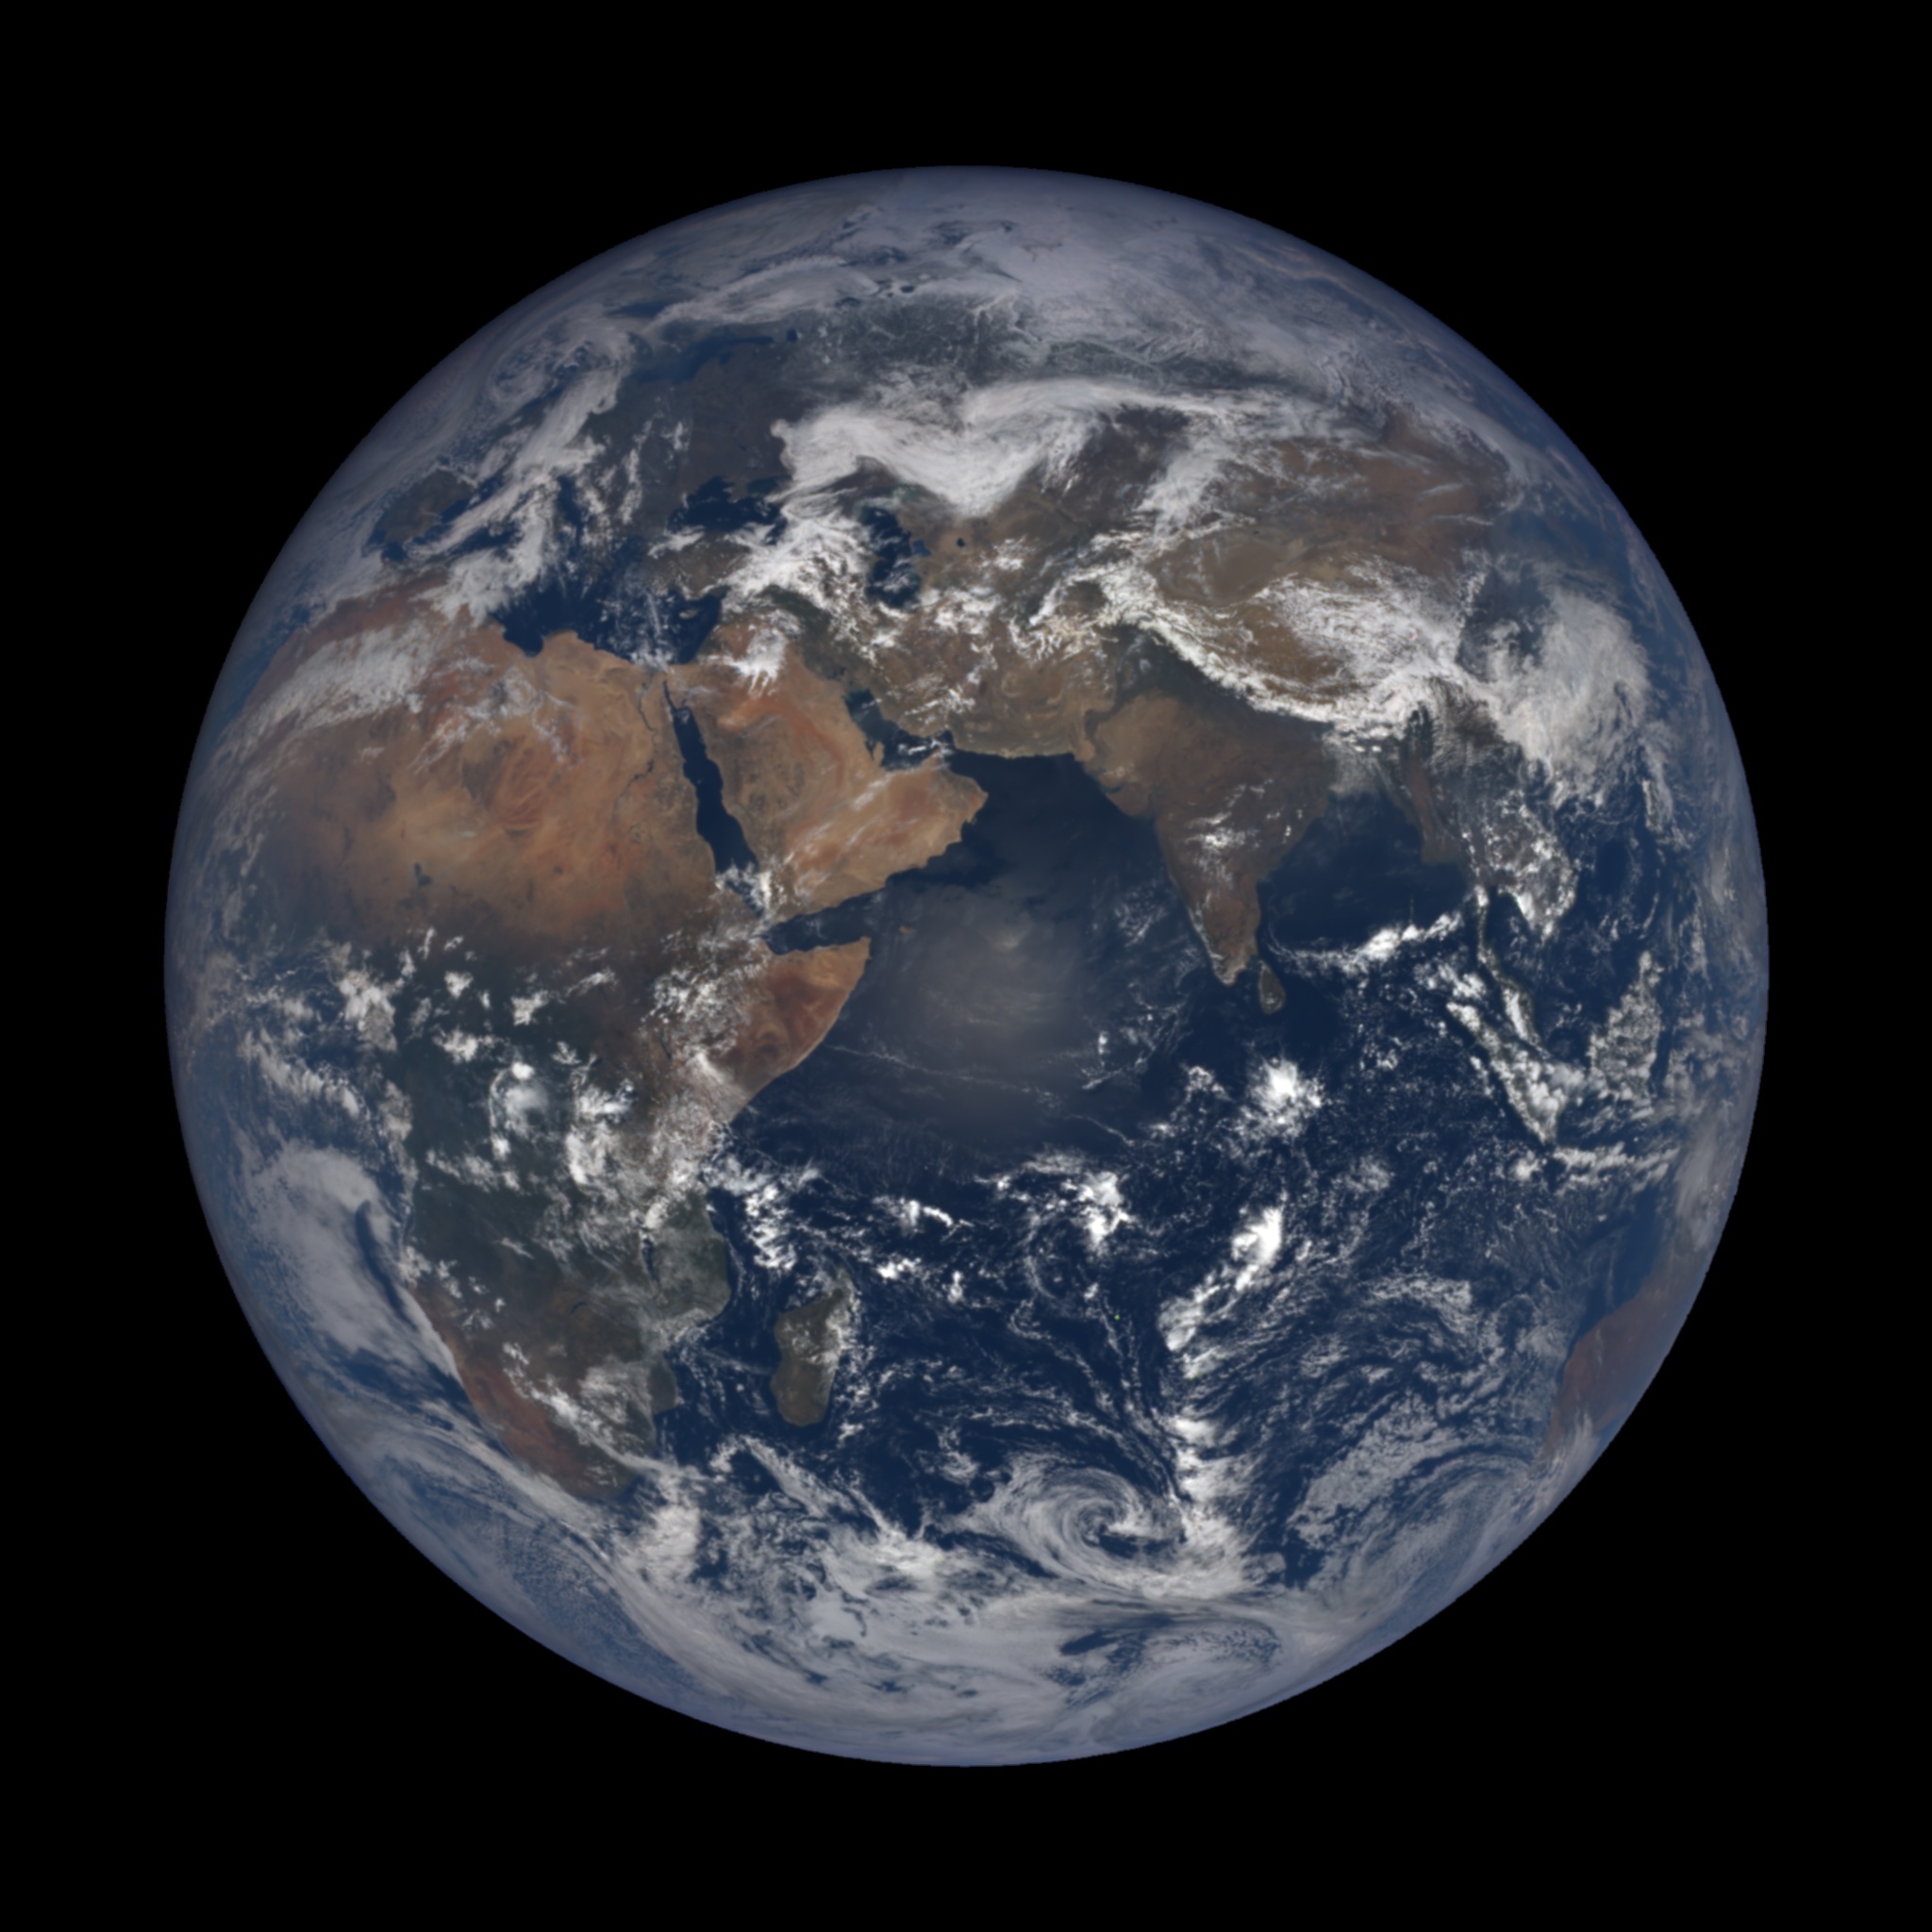
\includegraphics[width=5cm]{images/epic1}
			%\includegraphics[width=7cm]{images/fdl}
		\end{columns}
	\end{center}
	
	\vfill
\end{frame}
}


{\setbeamercolor{background canvas}{bg=tumbluedark}
	\begin{frame}[plain]
	
	\vfill
	\Huge\color{white}
	\begin{center}
		\begin{columns}
			\column{.5\textwidth}
			\vspace{7em}
			
			\hfill 
			Challenges
			\column{.5\textwidth}
			
			%			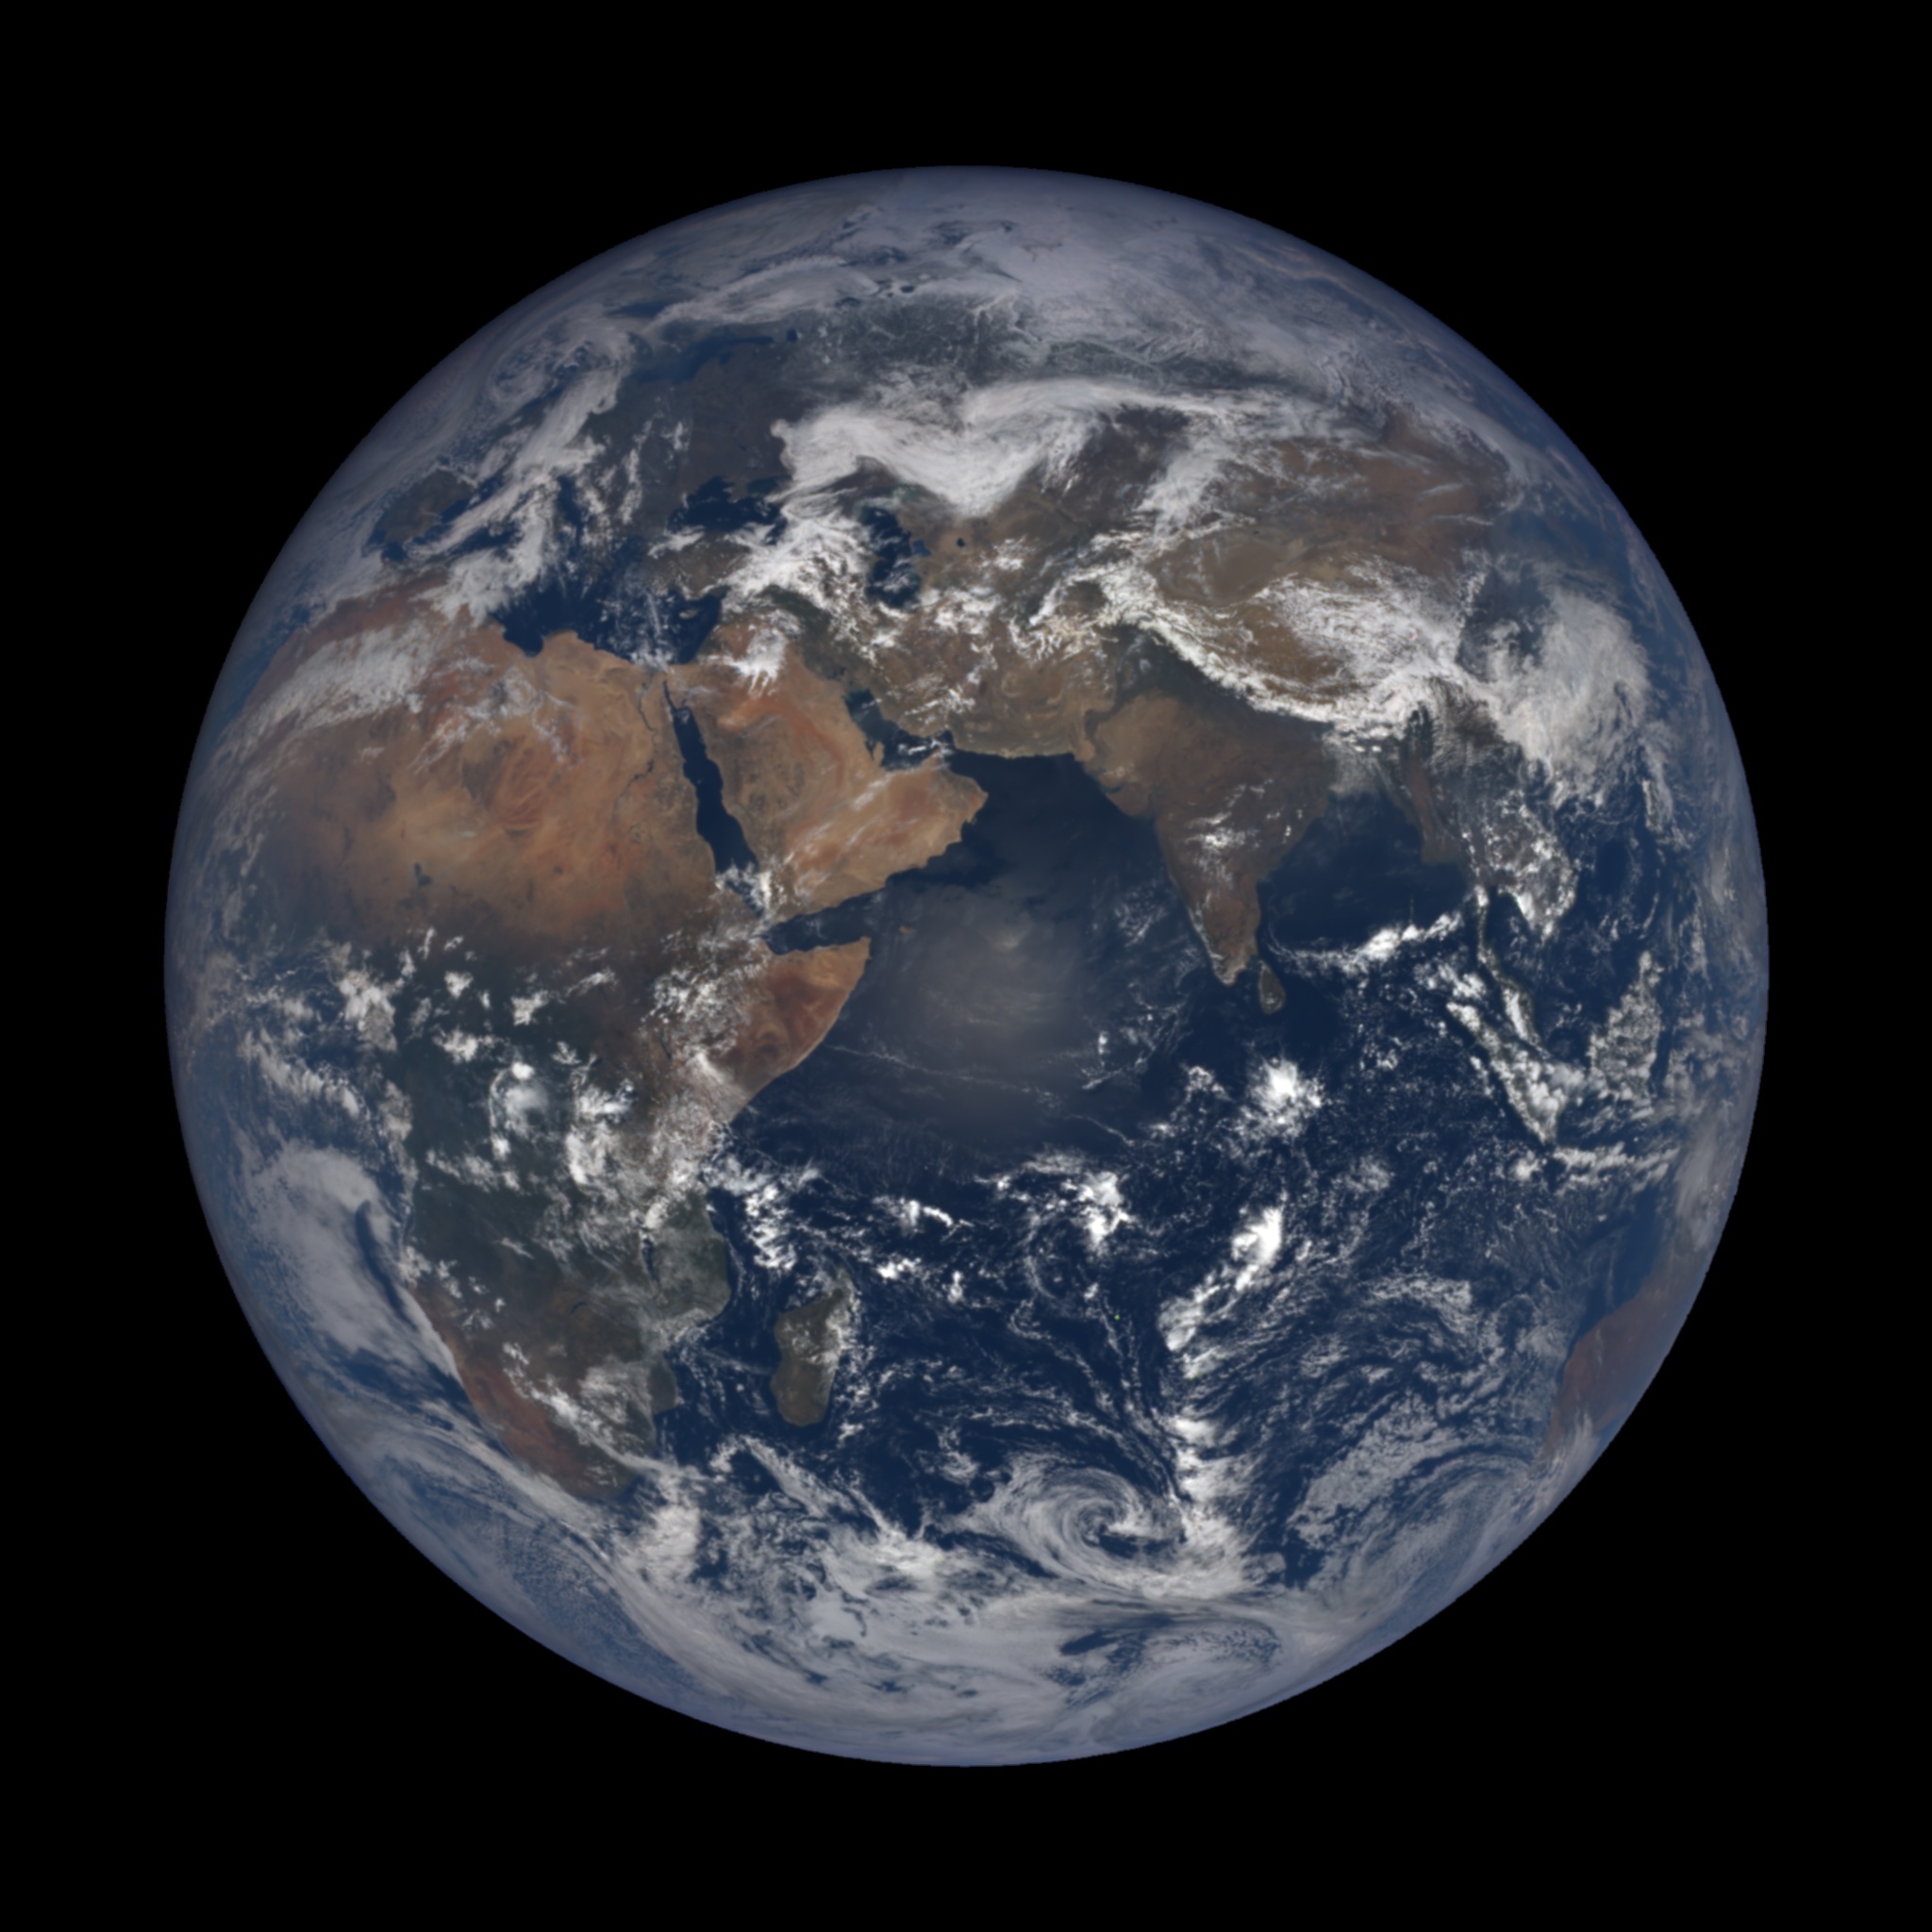
\includegraphics[width=5cm]{images/epic1}
			%\includegraphics[width=7cm]{images/fdl}
		\end{columns}
	\end{center}
	
	\vfill
\end{frame}
}



\begin{frame}
\frametitle{Challenge 1: Clouds adding a positive bias}

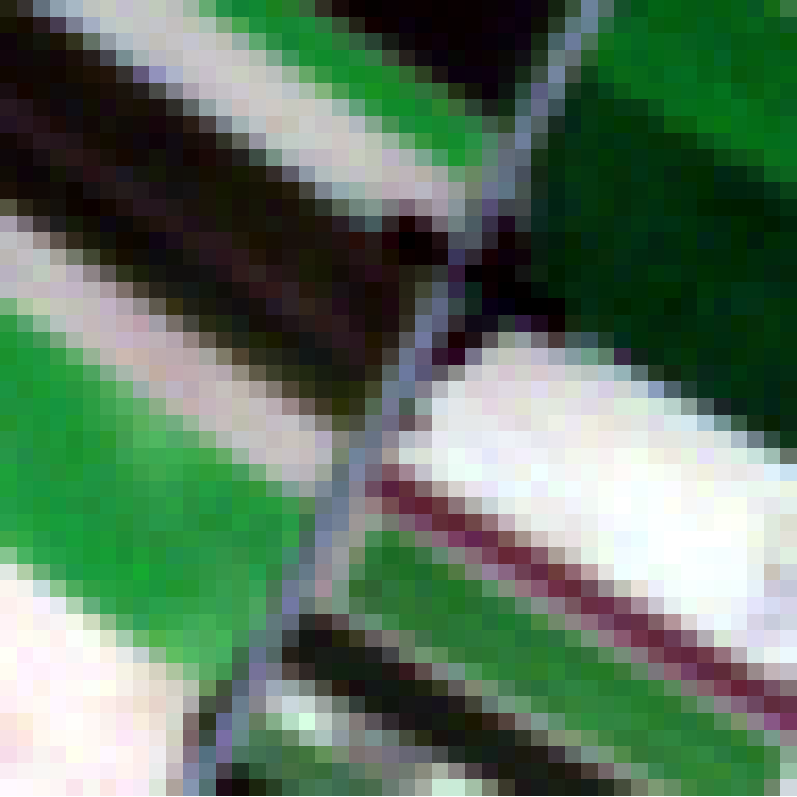
\includegraphics[width=2cm]{images/s2grid/1}
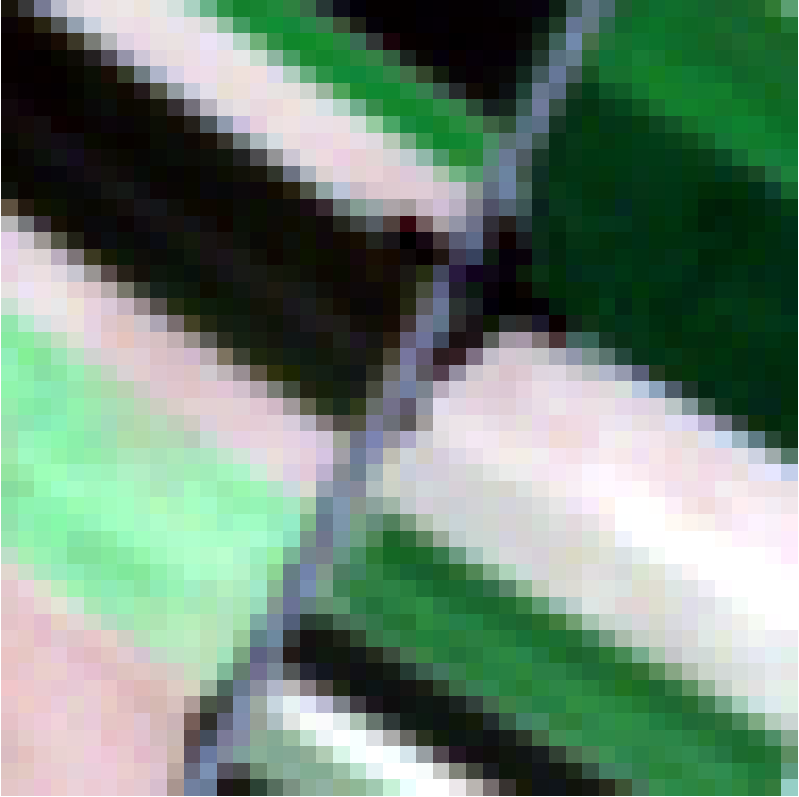
\includegraphics[width=2cm]{images/s2grid/2}

\includegraphics[width=2cm]{images/s2grid/3}

\includegraphics[width=2cm]{images/s2grid/4}

%\tikzsetnextfilename{example}

%\newcommand{\wv}[2]{$\lambda_\text{#1}=#2$}
\newcommand{\wv}[2]{$\rho_\text{#2}$}


\newcommand{\examplemeadows}{

\begin{tikzpicture}


\tikzstyle{annot} = [font=\tiny\sffamily, text=tumblue]
\tikzstyle{point} = [thin, tumbluelight, shorten >= .25em, shorten <= .25em]

% from /home/marc/projects/EV2019/images/example/tstop.txt
\def\tstopv{0.6285714285714286}
\def\class{winter barley}

\begin{axis}[date coordinates in=x,
date ZERO=2017-01-01,
xmin=2017-01-01,
xmax=2017-12-31,
ylabel near ticks,
ylabel style={font=\sffamily\small, rotate=0, yshift=-.5em},
width=.95\linewidth,
height=5cm,
axis x line=bottom,
axis y line=left,
%	enlarge x limits=0.01,
xtick={2017-01-01,2017-05-01,2017-08-01,2017-12-01},
xticklabels={January,April,August,December},
ymajorgrids,
ymax=10000,
thin,
smooth,
no marks,  
ylabel={$\rho \times 10^4$},
draw opacity=.8,
%		tension=0.001,
legend columns=8,
%y tick label style={rotate=90},
%legend to name=leg,
legend style={at={(.5,1.1)},anchor=south, line width=1pt, fill=tumblue!10}
]

%\addlegendimage{empty legend}


\addplot[b1color] table [x=doa, y=B1, col sep=comma] {images/example/3685593.csv};
\addplot[b2color] table [x=doa, y=B2, col sep=comma] {images/example/3685593.csv};
\addplot[b3color] table [x=doa, y=B3, col sep=comma] {images/example/3685593.csv};
\addplot[b4color] table [x=doa, y=B4, col sep=comma] {images/example/3685593.csv};
\addplot[b5color] table [x=doa, y=B5, col sep=comma] {images/example/3685593.csv};
\addplot[b6color] table [x=doa, y=B6, col sep=comma] {images/example/3685593.csv};
\addplot[b7color] table [x=doa, y=B7, col sep=comma] {images/example/3685593.csv};
\addplot[b8color] table [x=doa, y=B8, col sep=comma] {images/example/3685593.csv};
\addplot[b8Acolor] table [x=doa, y=B8A, col sep=comma] {images/example/3685593.csv};
\addplot[b9color] table [x=doa, y=B9, col sep=comma] {images/example/3685593.csv};
\addplot[b10color] table [x=doa, y=B10, col sep=comma] {images/example/3685593.csv};
\addplot[b11color] table [x=doa, y=B11, col sep=comma] {images/example/3685593.csv};
\addplot[b12color] table [x=doa, y=B12, col sep=comma] {images/example/3685593.csv};

%\node[above=of leg]{test};
%
%\addlegendentry{$\sqrt{x}$}
%\addlegendentry{$\ln{x}$}
%
%\addlegendentry[xshift=-10pt, font=\bfseries]{S2 Satellite Bands}

\addlegendentry{\wv{B01}{443nm}}
\addlegendentry{\wv{B2}{492nm}}
\addlegendentry{\wv{B3}{560nm}}
\addlegendentry{\wv{B4}{665nm}}
\addlegendentry{\wv{B5}{704nm}}
\addlegendentry{\wv{B6}{740nm}}
\addlegendentry{\wv{B7}{783nm}}
\addlegendentry{\wv{B8}{833nm}}
\addlegendentry{\wv{B8A}{864nm}}
\addlegendentry{\wv{B9}{945nm}}
\addlegendentry{\wv{B10}{1374nm}}
\addlegendentry{\wv{B12}{2202nm}}

%\legend{
%\wv{B01}{443nm},
%\wv{B2}{492nm},
%\wv{B3}{560nm},
%\wv{B4}{665nm},
%\wv{B5}{704nm},
%\wv{B6}{740nm},
%\wv{B7}{783nm},
%\wv{B8}{833nm},
%\wv{B8A}{864nm},
%\wv{B9}{945nm},
%\wv{B10}{1374nm},
%\wv{B11}{1613nm},
%\wv{B12}{2202nm}}


\end{axis}


%\node[font=\scriptsize\sffamily, anchor=west] at (0.2,2.7) {Sentinel 2 Satellite Spectral Bands};


\end{tikzpicture}
}


\newcommand{\examplecorn}{
	
	\begin{tikzpicture}
	
	\tikzstyle{annot} = [font=\tiny\sffamily, text=tumblue]
	\tikzstyle{point} = [thin, tumbluelight, shorten >= .25em, shorten <= .25em]
	
	% from /home/marc/projects/EV2019/images/example/tstop.txt
	\def\tstopv{0.6285714285714286}
	\def\class{winter barley}
	
	\begin{axis}[date coordinates in=x,
	date ZERO=2017-01-01,
	xmin=2017-01-01,
	xmax=2017-12-31,
	ylabel near ticks,
	ylabel style={font=\sffamily\small, rotate=0, yshift=-.5em},
	width=.95\linewidth,
	height=5cm,
	axis x line=bottom,
	axis y line=left,
	%	enlarge x limits=0.01,
	xtick={2017-01-01,2017-05-01,2017-08-01,2017-12-01},
	xticklabels={January,April,August,December},
	ymajorgrids,
	ymax=10000,
	thin,
	smooth,
	no marks,  
	ylabel={$\rho \times 10^4$},
	draw opacity=.8,
	%		tension=0.001,
	legend columns=8,
	%y tick label style={rotate=90},
	legend style={at={(.5,1)},anchor=south, line width=1pt, fill=tumblue!10}
	]
	
	
	\addplot[b1color] table [x=doa, y=B1, col sep=comma] {images/example/6139251.csv};
	\addplot[b9color] table [x=doa, y=B9, col sep=comma] {images/example/6139251.csv};
	\addplot[b10color] table [x=doa, y=B10, col sep=comma] {images/example/6139251.csv};
	
	\addplot[b11color] table [x=doa, y=B11, col sep=comma] {images/example/6139251.csv};
	\addplot[b12color] table [x=doa, y=B12, col sep=comma] {images/example/6139251.csv};
	
	\addplot[b5color] table [x=doa, y=B5, col sep=comma] {images/example/6139251.csv};
	\addplot[b6color] table [x=doa, y=B6, col sep=comma] {images/example/6139251.csv};
	\addplot[b7color] table [x=doa, y=B7, col sep=comma] {images/example/6139251.csv};
	\addplot[b8color] table [x=doa, y=B8, col sep=comma] {images/example/6139251.csv};
	\addplot[b8Acolor] table [x=doa, y=B8A, col sep=comma] {images/example/6139251.csv};
	
	\addplot[b2color] table [x=doa, y=B2, col sep=comma] {images/example/6139251.csv};
	\addplot[b3color] table [x=doa, y=B3, col sep=comma] {images/example/6139251.csv};
	\addplot[b4color] table [x=doa, y=B4, col sep=comma] {images/example/6139251.csv};
	
	\node[font=\sffamily] at (rel axis cs:0.35,0.9)(gr){ground signal};
	\draw (gr) -- (rel axis cs:.26,.3);
	\draw (gr) -- (rel axis cs:.2,.3);
	\draw (gr) -- (rel axis cs:.4,.25);
	
	\node[font=\sffamily] at (rel axis cs:0.8,.93)(cl){cloud noise};
	
	\draw (cl) -- (rel axis cs:.68,.7);
	\draw (cl) -- (rel axis cs:.58,.7);
	\draw (cl) -- (rel axis cs:.81,.7);
	
%	\legend{3 atmospheric, 2 short-wave infrared, 5 near infrared, 3 visible bands}
%	
	
	\addlegendentry{\wv{B01}{443nm}}
	\addlegendentry{\wv{B2}{492nm}}
	\addlegendentry{\wv{B3}{560nm}}
	\addlegendentry{\wv{B4}{665nm}}
	\addlegendentry{\wv{B5}{704nm}}
	\addlegendentry{\wv{B6}{740nm}}
	\addlegendentry{\wv{B7}{783nm}}
	\addlegendentry{\wv{B8}{833nm}}
	\addlegendentry{\wv{B8A}{864nm}}
	\addlegendentry{\wv{B9}{945nm}}
	\addlegendentry{\wv{B10}{1374nm}}
	\addlegendentry{\wv{B12}{2202nm}}
	

	\end{axis}
	
	\end{tikzpicture}
}
\examplecorn

\end{frame}

\begin{frame}
\frametitle{Challenge : Imbalanced class labels}

%\tikzsetnextfilename{partition_histograms}
\begin{tikzpicture}
  \begin{axis}[
  		thick,
        ybar, 
        axis on top,
        title={},
        height=7cm, width=.9\textwidth,
        bar width=.3em,
        ymajorgrids, 
        tick align=outside,
%        major grid style={draw=tumwhite},
%        enlarge y limits={value=.1,upper},
        ymin=0,
%        axis x line*=bottom,
%        axis y line*=left,
        ymode=log,
        axis line style={opacity=1, thin},
%        tickwidth=1pt,
        enlarge x limits=.05,
        ylabel={Parcels},
        ylabel style={yshift=0em},
%        xlabel style={yshift=2em},
%        x tick label style={yshift=-1em},
        xtick={0,2,...,12},
        xticklabels={barley, corn\phantom{g}, fallow, orchards, permanent meadows, rapeseed, vegetables},
        every x tick/.style={text height=1ex},
        extra x ticks={1,3,...,11},
        extra x tick labels={wheat, fodder, miscellaneous, cereals, protein crops, temporary meadows},
        every extra x tick/.style={major tick length=1em,
        	text height=1ex}
%        tick label style={rotate=20,anchor=east}
%        x tick label style={align=right,text width=3.5cm},
%       xticklabel style = {rotate=90,anchor=east},
       %nodes near coords={
       % \tiny \pgfmathprintnumber[precision=0]{\pgfplotspointmeta}
       %}
    ]
    
    \addplot [draw=none, fill=frh01color] table[x=id,y=frh01, col sep=comma] {images/counts.csv};
    \addplot [draw=none, fill=frh02color] table[x=id,y=frh02, col sep=comma] {images/counts.csv};
    \addplot [draw=none, fill=frh03color] table[x=id,y=frh03, col sep=comma] {images/counts.csv};
    \addplot [draw=none, fill=frh04color] table[x=id,y=frh04, col sep=comma] {images/counts.csv};

    \legend{Côtes-d’Armor {(FRH01)},Finistère {(FRH02)},Ille-et-Vilaine {(FRH03)},Morbihan {(FRH04)}}
  \end{axis}
  
%  \node at (20,2){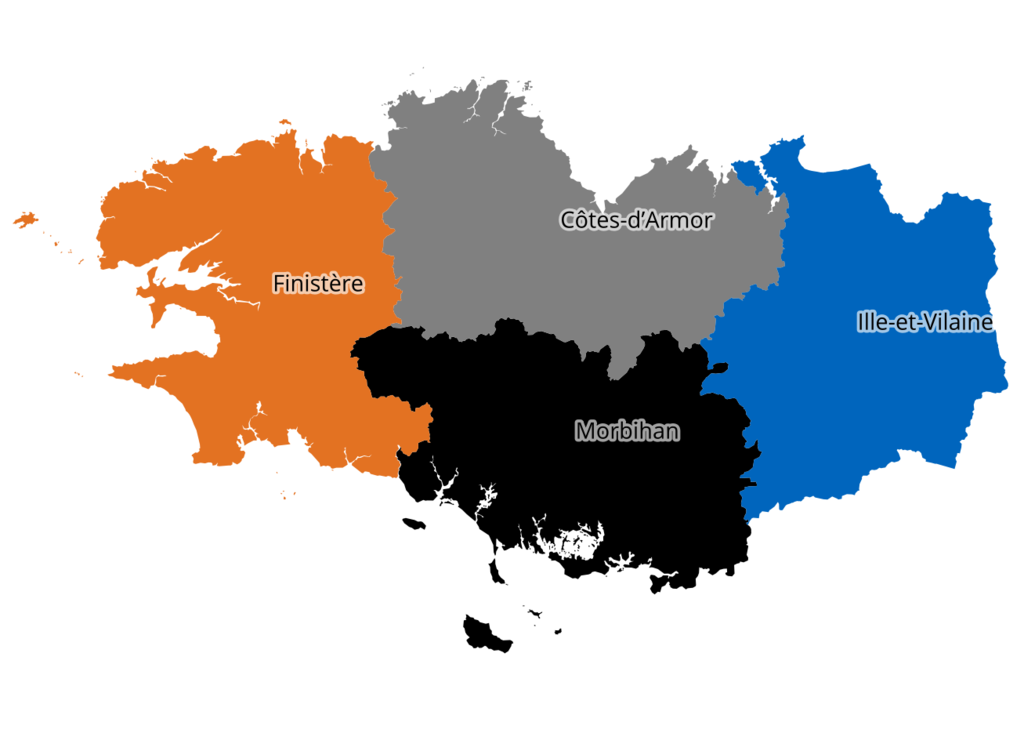
\includegraphics[width=8cm]{images/map/regions}};
  \end{tikzpicture}
\end{frame}

\begin{frame}
\frametitle{Challenge: Classes with similar characteristics}

Multi-Layer RNN baseline

\begin{columns}

\column{.5\textwidth}
\textbf{Precision}

\confmat{images/data/BreizhCrops_rnn/npy/confmat_flat.csv}{3}{1}

\column{.5\textwidth}
\textbf{Recall}

\confmat{images/data/BreizhCrops_rnn/npy/confmat_flat.csv}{4}{1}

\end{columns}

\end{frame}

%
%\begin{frame}
%\frametitle{Transformer baseline}
%
%\newcommand{\confmat}[3]{

\begin{tikzpicture}

  \def\vmax{#3}
  \def\dataindex{#2}
  
%
%  \pgfplotsset{every axis label/.append style={font=\footnotesize},tick pos=right, ylabel near ticks}
%  
%  \pgfplotsset{
%    axis line style={%
%      opacity=0 
%    }   
%  }

  \begin{groupplot}[
  	group style={
  		group size=2 by 1,
  		xlabels at=edge bottom,
  		ylabels at=edge left,
  		xticklabels at=edge bottom,
  		vertical sep=35pt,
  		group name=seq_len_plot
  	},
  	axis line style={draw=none},
  	title style={yshift=.75em,},
    width=6cm,
    height=6cm,
    enlargelimits=false,
    xtick=data,
%     ymin=1,
    xtick distance=1,
    ytick distance=1,
    colormap={example}{%
		color=(tumwhite)%color=(tumbluelight)
%		color=(tumivory)
%		color=(tumorange)
		color=(tumblue)%color=(tumbluelight)
%		color=(tumblack)
	},
    ytick=data,
    ytick align=outside,
    xtick align=outside,
%    tick style={draw=none},
    ytick pos = left,  
    tick label style = {font=\tiny\sansmath\sffamily},
    %xticklabel = {xshift=-0.75cm}
    yticklabel pos=left,
    %yticklabel near ticks,
    xlabel={\normalsize predicted},
    xlabel style={yshift=1em},
    ylabel style={yshift=-3em},
    x label style={at={(axis description cs:0.5,1)},anchor=south},
    y label style={at={(axis description cs:-0.1,.5)},anchor=south},
    ylabel={\normalsize ground truth},
%     ylabel near ticks,
%    xticklabels={},
  ]
  \nextgroupplot[
%      yticklabels={
%%      	{sugar beet},
%%      	{summer oat},
%%      	{meadow},
%%      	{rape},
%%      	%{vegetable},
%%      	{hop},
%%      	{winter spelt},
%%      	{winter triticale},
%%      	{beans},
%%      	{peas},
%%      	{potato},
%%      	{soybeans},
%%      	{asparagus},
%%      	{winter wheat},
%%      	{winter barley},
%%      	{winter rye},
%%      	{summer barley},
%%      	{maize}
%      },
%      xticklabels={
%%      	{sug.},
%%      	{s. oat},
%%      	{mead.},
%%      	{rape},
%%      	%{vegetable},
%%      	{hop},
%%      	{w. spelt},
%%      	{w. trit.},
%%      	{beans},
%%      	{peas},
%%      	{potato},
%%      	{soyb.},
%%      	{asp.},
%%      	{w. wheat},
%%      	{w. barley},
%%      	{w. rye},
%%      	{s. barley},
%%      	{maize}
%      },
     %colorbar style={title={\precisionrecall}, xshift=0cm, font=\footnotesize},
     colorbar right,
     colorbar style={
        	title={}, 
        	font=\footnotesize,
        	%at={(0,1)},
        	anchor=north west,
        	width=8pt,
        	ticklabel pos=right,
        	ticklabel style={xshift=2em},
%        	label style={yshift=-1em},
        	rounded corners=1pt
     },
  ]
  
    \addplot[
      matrix plot,
%      draw=tumwhite,
%       nodes near coords=\coordindex,
%       nodes near coords align={center},
%       nodes near coords style={font=\scriptsize},
        shader=faceted,
        faceted color=tumgraylight!20,
%       shader=faceted interp,
      mesh/cols=13,
      empty line=scanline,
      point meta=explicit,
      point meta min=0,
      point meta max=\vmax,
    ] table[meta index=\dataindex] {#1};
%   \nextgroupplot[
%       title=2017,
%       %colorbar style={title={\precisionrecall}, xshift=0cm, font=\footnotesize},
%       colorbar right,
%       colorbar style={
%       	title={a}, 
%       	font=\footnotesize,
%       	%at={(0,1)},
%       	anchor=north west,
%       	width=8pt,
%       	ticklabel pos=right,
%       	ticklabel style={xshift=1em},
%       	label style={yshift=1em},
%       	rounded corners=1pt
%       },
%       yticklabels={},
%     xticklabels={
%           	{sug.},
%           	{s. oat},
%           	{mead.},
%           	{rape},
%           	%{vegetable},
%           	{hop},
%           	{w. spelt},
%           	{w. trit.},
%           	{beans},
%           	{peas},
%           	{potato},
%           	{soyb.},
%           	{asp.},
%           	{w. wheat},
%           	{w. barley},
%           	{w. rye},
%           	{s. barley},
%           	{maize}
%     },
%       ]
%    
%    \addplot[
%    matrix plot,
%%    draw=tumwhite,
%    ,   
%    %       nodes near coords=\coordindex,
%    %       nodes near coords align={center},
%    %       nodes near coords style={font=\scriptsize},
%    shader=faceted,
%    faceted color=tumgraylight,
%    %       shader=faceted interp,
%    mesh/cols=17,
%    empty line=scanline,
%    point meta=explicit,
%    point meta min=0,
%    point meta max=\vmax,
%    ] table[meta index=\dataindex] {images/confmat/formatted_grucm2017.csv};
    
  \end{groupplot}
\end{tikzpicture}
}
%
%\begin{columns}
%
%\column{.5\textwidth}
%\confmat{images/data/BreizhCrops_transformer/npy/confmat_flat.csv}{3}{1}
%
%\column{.5\textwidth}
%\confmat{images/data/BreizhCrops_transformer/npy/confmat_flat.csv}{4}{1}
%
%\end{columns}
%
%\end{frame}


\begin{frame}
\frametitle{Challenge: Irregular sampling distance.}

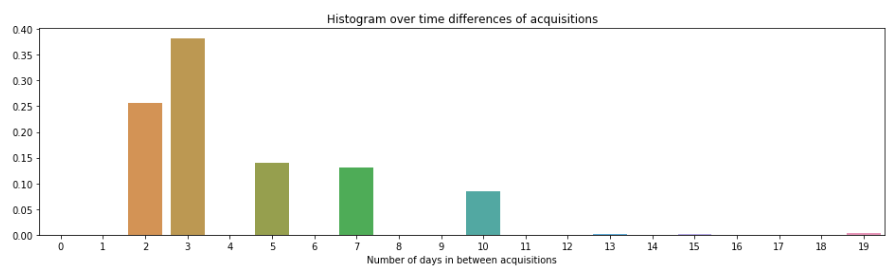
\includegraphics[width=\textwidth]{images/days_between_acquisitions}

\end{frame}

\begin{frame}
\frametitle{Challenge: Variable sequence length}
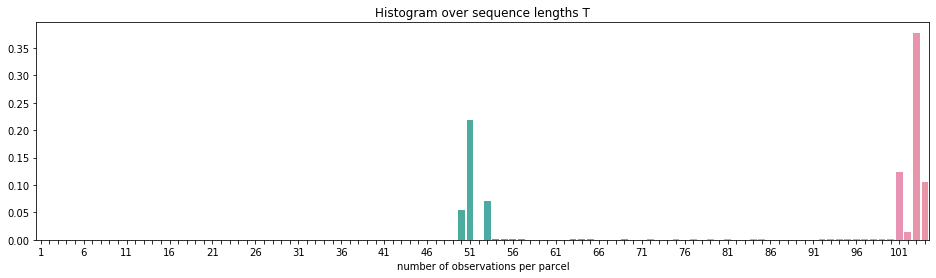
\includegraphics[width=\textwidth]{images/sequencelengths}

\end{frame}



\begin{frame}
\frametitle{Challenge: Regional variations in the class distributions}



\begin{tikzpicture}
\node(o){\includegraphics[width=2.5cm]{images/orchards}};

\coordinate[yshift=2.55cm](co2) at (o);
\draw ($ (co2)+(-1cm,0) $) -- ($ (co2)+(1cm,0) $) node[name=labblue, pos=1.1, anchor=west]{1224 parcels};

\coordinate[yshift=-.43cm](co) at (o);
\draw ($ (co)+(-1cm,0) $) -- ($ (co)+(1cm,0) $) node[name=laborange, pos=1.1, anchor=west]{350 parcels};

\node[right=4cm of o](regions){\includegraphics[width=8cm]{images/map/regions}};

\draw (laborange) -- ($ (regions)+(-2cm,.5cm) $);
\draw (labblue) -- ($ (regions)+(3cm,0cm) $);

\end{tikzpicture}

\end{frame}

\begin{frame}
\frametitle{Spatial autocorrelation}

\includegraphics[width=11cm]{images/map/breizh}


\end{frame}

{\setbeamercolor{background canvas}{bg=tumbluedark}
\begin{frame}[plain]

\vfill
\Huge\color{white}
\begin{center}
\begin{columns}
\column{.5\textwidth}
\vspace{7em}

\hfill 
Summary and Outlook
\column{.5\textwidth}

%			\includegraphics[width=5cm]{images/epic1}
%\includegraphics[width=7cm]{images/fdl}
\end{columns}
\end{center}

\vfill
\end{frame}
}



\begin{frame}
\frametitle{Scaling up}

\includegraphics[width=5cm]{images/EuroCrops}
\includegraphics[width=5cm]{images/France}
\includegraphics[width=4cm]{images/Bavaria}

\end{frame}

\begin{frame}
\frametitle{Supported by Google Research Credits}

\includegraphics[width=.3\textwidth]{images/google_research_credits}
\includegraphics[width=.3\textwidth]{images/google}
\includegraphics[width=.2\textwidth]{images/earth-engine-logo}
%\includegraphics[width=3cm]{images/250px-Google-Cloud-Storage-Logo}
%\includegraphics[width=3cm]{images/Google_Compute_Engine_logo}
%\includegraphics[width=3cm]{images/google_cloud_sql}


\end{frame}


\newcommand{\myvec}[1]{\ensuremath{\begin{pmatrix}#1\end{pmatrix}}}
\begin{frame}
\frametitle{Spatial and Temporal Discretization}

\begin{columns}
	\column{.5\textwidth}
	
	{
		\begin{equation*}
		\V{x}_t = \myvec{\rho_{\lambda_1} \\ \rho_{\lambda_2} \\ \dots \\ \rho_{\lambda_n}}
		\end{equation*}
	}
	
	
	
	Spectral reflectance of \textbf{spectral bands} disctretized on a \textbf{spatial grid}. Each grid cell is georeferenced by its Longitude $\Lambda$ and Latitude $\Phi$.
	Acquisitions in regular \textbf{temporal intervals}.
	
	\column{.5\textwidth}
	
	
	
	\begin{tikzpicture}
	
	%	\node(a){\includegraphics[width=3cm]{images/s2grid/1}};
	
	%	\draw[step=1cm,gray,very thin] (-2,-2) grid (6,6);
	
	
	\draw [fill=tumivory,domain=110:70] plot ({11*cos(\x)}, {11*sin(\x)-8.5});
	
	\begin{scope}[scale=1]
	
	% raster size
	\def\d{1}		
	
	% distance layer
	\def\s{\d*50}
	
	\node at (-1.7,2.4){$t_{i-1}$};
	\node at (-1.7,4.2){$t_i$};
	\node at (-1.7,6){$t_{i-1}$};
	
	\node at (1,1.9){$\Lambda$};
	\node at (-1,1.9){$\Phi$};
	
	%		\draw[step=1.0,black,thin] (-2,0) grid (2,5);
	
	
	\foreach \i in {1,...,3}
	{		
		
		\begin{scope}[
		yshift=\s*\i,every node/.append style={
			yslant=0.5,xslant=-1},yslant=0.5,xslant=-1,scale=0.35
		]
		%\draw[step=3.33mm] (0,0) grid (1,1);
		%\fill[black,fill opacity=.9] (0.333,0.333) rectangle (0.333,0.333);    	    	  
		
		
		
		\foreach \row in {0,...,3}{
			\foreach \col in {0,...,3}{
				\draw[tumblack, fill=tumblue!\pdfuniformdeviate 40,fill opacity=1,rounded corners=1] (\col,\row) rectangle (\col+1, \row+1);
				
				\node[font=\tiny, text=tumblue] at (\col + 0.5,\row + 0.5) {$\V{x}$};
				
				%                 \draw[black, fill=black!\pdfuniformdeviate 40,fill opacity=1,rounded corners=1] (\col*\d/3,\row*\d/3) rectangle (\col*\d/3+\d/3, \row*\d/3+\d/3);
			}
		}
		
		%\draw[step=3.33mm] (0,0) grid (1,1);
		%\fill[white,fill opacity=.9] (0,0) rectangle (1,1);
		\end{scope}
	}
	\end{scope}
	
	
	
	\end{tikzpicture}
	
\end{columns}


\end{frame}


\begin{frame}

\frametitle{Photosynthesis}
%	
%	Photosynthesis

\centering
\begin{tikzpicture}
\node(in){$6{\text{CO}}_{2}+6{\text{H}}_{2}\text{O}$};
\node[right=of in, label={light absorbtion $\Delta \V{x}$}](arrow){$\to$};
\node[right=of arrow]{${\text{C}}_{\text{6}}{\text{H}}_{\text{12}}{\text{O}}_{\text{6}}+{\text{6O}}_{\text{2}}$};
\end{tikzpicture}
%	
%	\begin{equation*}
%	6{\text{CO}}_{2}+6{\text{H}}_{2}\text{O}\to 
%	\end{equation*}
\end{frame}


\begin{frame}
\frametitle{Meadow Example}
\examplemeadows
\end{frame}


\begin{frame}
\frametitle{Sentinel 2: Satellite Time Series $\M{X} = (\V{x}_1,\V{x}_2,\dots,\V{x}_N)$}

\begin{columns}
	
	
	\column{.5\textwidth}
	
	\includegraphics[width=\textwidth]{images/sentinel2}
	
	\column{.5\textwidth}
	
	
	
	
	\begin{equation*}
	\V{x}_t = \begin{pmatrix}
	\rho_{UV} \\ 
	\rho_{Blue} \\
	\rho_{Green} \\
	\rho_{Red} \\
	\rho_{NIR} \\
	\rho_{NIR} \\
	\rho_{NIR} \\
	\rho_{NIR} \\
	\rho_{NIR} \\
	\rho_{SWIR} \\
	\rho_{SWIR} \\
	\rho_{SWIR} \\
	\rho_{SWIR}
	\end{pmatrix}
	%	\begin{matrix}
	%%	\leftarrow \text{ultra-violett} \\ 
	%%	\leftarrow \text{blue} \\
	%%	\leftarrow \text{green} \\
	%%	\leftarrow \text{red} \\
	%%	\leftarrow \text{near infrared} \\
	%%	\leftarrow \text{near infrared} \\
	%%	\leftarrow \text{near infrared} \\
	%%	\leftarrow \text{near infrared} \\
	%%	\leftarrow \text{near infrared} \\
	%%	\leftarrow \text{water vapour} \\
	%%	\leftarrow \text{detect cirrus clouds} \\
	%%	\leftarrow \text{short-wave infrared} \\
	%%	\leftarrow \text{short-wave infrared}
	%%\multirow{3}{c}{\overbrace{\rule{1.5cm}{0pt}}^{N(k,d)-d}}
	%\multirow{5}{*}{fractionals}
	%	\end{matrix}
	\end{equation*}
	\small UV=ultra-violet, NIR=near infra-red, SWIR=short-wave infra-red
\end{columns}

\end{frame}


\begin{frame}
\frametitle{Two Research Fields}
\centering
\begin{tikzpicture}[xscale=3.5, yscale=2]
%\draw[fill=tumblue, draw=none, opacity=0.5](-1,0) circle (1.5);
\node[fill=tumbluelight, draw=none, opacity=0.5, circle, minimum width=6cm, text opacity=1, font=\Large\bfseries] at (-1,0){Earth Observation};

\node[fill=tumorange!50, draw=none, opacity=0.5, circle, minimum width=6cm, text opacity=1, font=\Large\bfseries] at (1,0){Machine Learning};
%\draw[fill=tumorange, draw=none, opacity=0.5](1,0) circle (1.5);

%\node at (-1.3,1){Data};
%
%\node[text width=3.5cm] at (-1,.9){\focusmethod is a \textbf{tool} for our \focusdata};
%\node[text width=3.5cm] at (1,.9){\focusdata is a \textbf{benchmark} for our \focusmethod};
%
%
%\node[text width=3.5cm] at (-1,.3){\textbf{should generalize} to applications of a \\ specific sub-field};
%\node[text width=3.5cm] at (1,.3){\textbf{must generalize} to many fields of applications};
%
%\node[text width=3.5cm] at (-1,-.3){data has specific \\ \textbf{phyisical properties}};
%\node[text width=3.5cm] at (1,-.3){data is a \textbf{feature vector}};
%
%\node[text width=2cm] at (-1.3,-.6){{physics}, {sensors}, {applications}};

%\node at (1.3,1){Method};

%\node at (-1.3,1){IGARSS};
%\node at (-1.6,-1){ISPRS};
%\node at (-1.2,-.6){IEEE-GRSS};
%\node at (-1.8,.4){MDPI-RS Journal};
%\node at (-1.3,0){RSE Journal};
%
%\node at (1.3,1){NeurIPS};
%\node at (1.6,-1){CVPR};
%\node at (1.2,-.6){ICML};
%\node at (1.8,.4){ECCV};
%\node at (1.3,.2){ECML};
%
%\node at (0,.5){CVPR EarthVision};
%\node at (0,0){ECML MACLEAN};
%\node at (0,-.5){(ESA-$\Phi$-week)};

\end{tikzpicture}

\end{frame}


\begin{frame}
\frametitle{Common Datasets}
\centering
\begin{tikzpicture}[scale=2]
%\draw[fill=tumblue, draw=none, opacity=0.5](-1,0) circle (1.5);
\node[fill=tumbluelight, draw=none, opacity=0.5, circle, minimum width=6cm, label=Earth Observation] at (-.8,0){};

\node[fill=tumorange!50, draw=none, opacity=0.5, circle, minimum width=6cm, label=Machine Learning] at (.8,0){};
%\draw[fill=tumorange, draw=none, opacity=0.5](1,0) circle (1.5);

\node[font=\Large\bfseries, text width=2cm] at (0,0) {Common Datasets};

\end{tikzpicture}
\end{frame}



\end{document}



